% !Mode:: "TeX:UTF-8"
%\documentclass[a4paper, 12pt]{article}

\documentclass[twoside]{linux_thesis}
\usepackage{latexsym,bm}
\usepackage{amsmath}
\usepackage{amsfonts}
\usepackage{graphicx}
\usepackage{color}
\usepackage{setspace}
\usepackage{graphicx}
\usepackage{fontspec}
\usepackage{supertabular}

\linespread{1.3}

\begin{document}

\begin{center}
  \LARGE \textbf{Linux 学习笔记}
\end{center}

\newcommand{\shell}[1]{\noindent\texttt{\$: #1}}

\tableofcontents

\section{文件权限与目录配置}

\subsection{属性与权限}
\begin{itemize}
    \item \textbf{\texttt{chgrp}}: 改变文件所属用户组 \\
    \mbox{\qquad \texttt{chgrp [-R] dirname/filename}} \\
    参数 \texttt{-R} 表示进行递归修改.
    
    \item \textbf{\texttt{chown}}: 改变文件所有者\\
    \mbox{\qquad \texttt{chown [-R] 账号名称 dirname/filename}} \\
    \mbox{\qquad \texttt{chown [-R] 账号名称:组名 dirname/filename}} \\
    参数 \texttt{-R} 表示进行递归修改.
    
    \item \textbf{\texttt{chmod}}: 改变文件的权限\\
    \mbox{\qquad \texttt{chmod [-R] xyz dirname/filename}} \\
    或符号用法
    \begin{longtable}{c|c|c|c|c}\hline\hline
                                        & \texttt{u} &  &  &  \\
                                        & \texttt{g} & \raisebox{2.3ex}[0pt]{\texttt{+}} &  \raisebox{2.3ex}[0pt]{\texttt{r}} &  \\
\raisebox{2.3ex}[0pt]{\texttt{chmode}}  & \texttt{o} & \raisebox{2.3ex}[0pt]{\texttt{-}} &  \raisebox{2.3ex}[0pt]{\texttt{x}} & \raisebox{2.3ex}[0pt]{文件或目录} \\

                                        & \texttt{a} & \raisebox{2.3ex}[0pt]{\texttt{=}} &  \raisebox{2.3ex}[0pt]{\texttt{x}} & \\
    \hline
    \end{longtable}
\end{itemize} 

\subsection{目录配置}
1. FHS 标准
\begin{longtable}{c|p{0.8\columnwidth}}\hline
\textbf{目录} & \makebox[0.8\columnwidth]{\textbf{应放置的文件内容}}\\\hline
\endhead

\texttt{/bin} & 系统的执行文件. 单用户维护模式也可操作.\\

\texttt{/boot} & 开机会使用到的文件,包括 Linux 内核文件以及开机菜单与开机配置文件等.\\

\texttt{/dev} & 任何设备与接口设备都以文件形式存在于这个目录中. 比较重要的文件有 \texttt{/dev/null, /dev/zero, /dev/tty, /dev/hd*} 等.\\

\texttt{/etc} & 系统的主要配置文件, 例如系统账号密码文件、各种服务的起始文件等.\\

\texttt{/home} & 默认的用户主文件夹\\

\texttt{/lib} & 开机用到的函数库,以及在 \texttt{/bin} 或 \texttt{/sbin} 下命令会调用的函数库.\\

\texttt{/media} & 放置的是可删除设备,包括光盘、DVD等都暂挂在此. 常见的如 \texttt{/media/cdrom} 等.\\

\texttt{/mnt} & 暂时挂载某些额外的设备,例如 U 盘. 常见如 \texttt{/mnt/flash} 等.\\

\texttt{/opt} & 第三方软件放置的目录, 如 KDE 等.\\

\texttt{/root} & 系统管理员的主文件夹.\\

\texttt{/sbin} & 包括开机、修复、还原系统所需的命令. 某些服务器软件放置到 \texttt{/usr/sbin} 中, 本机安装的软件所产生的系统执行文件放置到 \texttt{/usr/local/sbin} 中.\\

\texttt{/srv} & 一些网络服务所需数据目录.\\
\texttt{
/tmp} & 一般用户正在执行的程序的临时目录.\\

\hline
\end{longtable}

\par
2. 其余重要目录.
\begin{longtable}{c|p{0.8\columnwidth}}\hline
\textbf{目录} & \makebox[0.8\columnwidth]{\textbf{应放置的文件内容}}\\\hline
\endhead

\texttt{/lost+found} & 文件系统发生错误时,会将丢失的片段放置到该目录.\\

\texttt{/proc} & 虚拟文件系统,该目录数据都在内存中.较重要的文件如 \texttt{/proc/cpuinfo, /proc/dma} 等\\

\texttt{/sys} & 虚拟文件系统,记录与内核相关的信息,包括已加载的内核模块和检测到的硬件设备信息等. 不占硬盘容量.\\

\hline
\end{longtable}

\par
3. \texttt{/usr} 的内容与意义.
\begin{longtable}{c|p{0.8\columnwidth}}\hline
\textbf{目录} & \makebox[0.8\columnwidth]{\textbf{应放置的文件内容}}\\\hline
\endhead

\texttt{/usr/X11R6/} & X Window 系统重要数据放置目录. \\

\texttt{/usr/bin/} & 绝大部分用户可使用命令. \\

\texttt{/usr/include/} & 头文件与包含文件. \\

\texttt{/usr/lib/} & 包含应用软件的函数库、目标文件,以及不被一般用户惯用的执行文件或脚本.\\

\texttt{/usr/local/} & 系统管理员在本机安装自己下载的软件.\\

\texttt{/usr/sbin/} & 非系统正常运行所需要的系统命令,如某些网络服务器软件的服务命令.\\

\texttt{/usr/share/} & 共享文件. \\

\texttt{/usr/src/} & 一般源码. 内核源码建议放置在 /usr/src/linx/ 目录下.\\

\hline
\end{longtable}

\par
4. \texttt{/var} 的内容与意义.
\begin{longtable}{c|p{0.8\columnwidth}}\hline
\textbf{目录}\quad & \makebox[0.8\columnwidth]{\textbf{应放置的文件内容}}\\\hline
\endhead

\texttt{/var/cache/} &  应用程序的缓存文件. \\

\texttt{/var/lib/} &  程序本身执行的过程中,需要使用到的数据文件.例如, MySQL 的数据库放置到 \texttt{/var/lib/mysql/} 中.\\

\texttt{/var/lock/} &  将设备上锁,以确保文件只被单一软件使用. \\

\texttt{/var/log/} &  登录文件.\\

\texttt{/var/mail/} &  个人电子邮箱.\\

\texttt{/var/run/} &  某些程序启动后,会将他们的PID放置在该目录.\\

\texttt{/var/spool/} &  通常放置一些队列数据. \\

\hline
\end{longtable}

\section{文件与目录管理}
\subsection{管理}
\par
\textbf{1. 特殊目录}:
\begin{longtable}{l@{ : }p{0.4\columnwidth}}\hline\hline

  \texttt{.} & 当前目录\\

  \texttt{..} & 当前目录的上层目录 \\

  \texttt{-} & 前一个工作目录 \\

  \texttt{$\sim$} & 当前用户的主文件夹 \\

  \texttt{$\sim$yong} & 用户名为 yong 的主文件夹\\

  \hline
\end{longtable}

\textbf{2. 相关命令}:
\begin{itemize}
\item \textbf{\texttt{cd [相对路径或绝对路径(不加该参数同$\sim$)]}}: 切换目录.

\item \textbf{\texttt{pwd [-P]}}: 显示当前路径,参数 \texttt{-P} 表示不显示连接路径而显示完整路径.

\item \textbf{\texttt{mkdir}}: 新建目录
  \begin{longtable}{l@{: }p{0.7\columnwidth}}\hline\hline

    \textbf{用法} & \verb"mkdir [-mp] 目录名称"
    \\

    \texttt{-m} & 配置文件夹权限. 直接设置,不需要看默认权限(umask)  \\

     \texttt{-p}  & 递归创建目录 \\

    \hline
  \end{longtable}

\item \textbf{\texttt{rmdir}}: 删除空目录
  \begin{longtable}{l@{: }p{0.7\columnwidth}}\hline\hline

    \textbf{用法} & \verb"rmdir [-p] 目录名称"\\

     \texttt{-p}  & 连同上层空目录一并删除 \\

    \hline
  \end{longtable}

\item \textbf{\texttt{ls}}: 查看文件与目录
  \begin{longtable}{c@{: }p{0.7\columnwidth}}\hline\hline

    \textbf{用法} & \verb"ls [-aAdfFhilnrRSt] 目录名称" \newline
                    \verb"ls [--color={never,auto,always}] 目录名称" \newline
                    \verb"ls [--full-time] 目录名称"
    \\

    \texttt{-a} & 列出全部文件(含隐藏文件和 \texttt{.} 与 \texttt{..} 两个目录)  \\

     \texttt{-A}  &  和 \texttt{-a} 同, 但无\texttt{.} 与 \texttt{..} 两个目录  \\

    \texttt{-d} & 仅目录本身 \\

    \texttt{-f} & 不进行排序(默认会以文件名排序) \\

    \texttt{-F} & 根据文件,目录信息给予附加数据结构 \\

    \texttt{-h} & 将文件容量以易读方式列出 \\

    \texttt{-i} & 列出 inode 号码 \\

   \texttt{-l} & 列出长数据串, 包含文件属性与权限等数据 \\

    \texttt{-n} & 列出 UID 与 GID \\

    \texttt{-r} & 将排序结果反向输出 \\

    \texttt{-R} & 连同子目录内容一起列出 \\

    \texttt{-S} & 以文件容量大小排序 \\

    \texttt{-t} & 以时间排序 \\

    \texttt{--color=never} & 不依据文件特性给予颜色显示 \\

    \texttt{--color=always} & 显示颜色 \\

    \texttt{--color=auto} & 让系统自行判断 \\

    \texttt{--full-time} & 以完整时间模式输出 \\

    \texttt{--time={atime,ctime}} & 输出 ctime \\

    \hline
  \end{longtable}

\item \textbf{\texttt{cp}}: 复制
  \begin{longtable}{c@{: }p{0.7\columnwidth}}\hline\hline

    \textbf{用法} & \verb"cp [-adfilprsu] 源文件 目标文件" \newline
                    \verb"cp [options] 源文件1 源文件2 ... 目录"
    \\

    \texttt{-a} & 相当于 \texttt{-pdr}  \\

     \texttt{-d}  &  源文件为连接文件,则复制连接文件属性而非文件本身  \\

    \texttt{-f} & 强制 \\

    \texttt{-i} & 覆盖时先询问 \\

    \texttt{-l} & 进行硬连接,而非复制文件本身 \\

    \texttt{-p} & 连同文件的属性一起复制 \\

    \texttt{-r} & 递归复制 \\

   \texttt{-s} & 复制成 symbolic link \\

    \texttt{-u} & 当源文件更新时才复制 \\

    \hline
  \end{longtable}

\item \textbf{\texttt{rm}}: 移除文件或目录
  \begin{longtable}{c@{: }p{0.7\columnwidth}}\hline\hline

    \textbf{用法} & \verb"rm [-fir] 文件或目录"
    \\

    \texttt{-f} & 强制  \\

     \texttt{-i}  &  互动模式  \\

    \texttt{-r} & 递归删除 \\

    \hline
  \end{longtable}

\item \textbf{\texttt{mv}}: 移动文件与目录,或更名
  \begin{longtable}{c@{: }p{0.7\columnwidth}}\hline\hline

    \textbf{用法} & \verb"mv [-fiu] source destination" \newline
                    \verb"mv [options] source1 source2 ... destination"
    \\

    \texttt{-f} & 强制  \\

     \texttt{-i}  &  若覆盖先询问  \\

    \texttt{-u} & 若目标已存在,且source更新,才会更新 \\

    \hline
  \end{longtable}

\item \textbf{\texttt{basename}}: 取得路径的文件名

\item \textbf{\texttt{dirname}}: 获取目录名

\end{itemize}

\subsection{查阅文件内容}
\begin{itemize}

\item \textbf{\texttt{cat}}
  \begin{longtable}{c@{: }p{0.5\columnwidth}}\hline\hline

    \textbf{用法} & \verb"cat [-AbEnTv] 文件"
    \\

    \texttt{-A} & 相当于 \texttt{-vET}  \\

     \texttt{-b}  &  列出行号,空白行不标号  \\

    \texttt{-E} & 将结尾的断行符 \$ 显示出来 \\

     \texttt{-n} & 显示行号,包括空白行  \\

     \texttt{-T}  &  将[Tab]键以 \verb|^I| 显示  \\

    \texttt{-v} & 列出一些看不出来的特殊字符 \\

    \hline
  \end{longtable}

\item \textbf{\texttt{tac}}:反向显示

\item \textbf{\texttt{nl}}:显示行号(可设定行号格式和左右位置)

\item \textbf{\texttt{more}}:翻页查看

\item \textbf{\texttt{less}}:相比于 more, 功能更丰富

\item \textbf{\texttt{head [-n number] 文件}}: 取出前面几行

\item \textbf{\texttt{tail [-n number] 文件}}: 取出后面几行

\item \textbf{\texttt{od [-t TYPE(a,c,d,f,o,x)] 文件}}: 读取非纯文本文件

\item \textbf{\texttt{touch [-acdmt] 文件}}: 创建空文件或修改文件mtime, atime

\item \textbf{\texttt{file 文件}}: 查看文件类型

\end{itemize}

文件三个时间的意义:
\begin{itemize}
    \item \texttt{mtime(modification time)}: 文件内容更改时,会更新该时间.

    \item \texttt{ctime(status time)}:文件的状态改变时(如权限与属性等),会更新该时间.

    \item \texttt{atime(access time)}:文件内容被取用,会更新该时间.
\end{itemize}

\subsection{默认权限与隐藏权限}
\subsubsection{umask}
\texttt{umask} 可指定当前用户在新建文件或目录时权限的默认值.
\begin{itemize}
    \item \texttt{umask [分数]}: 设置默认权限.不加参数时,显示当前的分数,分数表示的是,创建文件或目录的默认值需要减掉的权限.

    \item \texttt{umask -S}: 符号显示当前的默认权限.
\end{itemize}

\subsubsection{隐藏属性}
\begin{itemize}
\item \texttt{chattr}:设置文件的隐藏属性
  \begin{longtable}{c@{: }p{0.9\columnwidth}}\hline\hline

    \textbf{用法} & \verb"chattr [+-=][ASacdistu] 文件或目录"
    \\

    \texttt{-A} & 访问该文件或目录时, atime 不会被修改  \\

     \texttt{-S}  & 对文件做任何修改都会同步写入磁盘  \\

    \texttt{-a} & \textbf{\kaishu 只能增加数据,不能删除和修改数据. root权限才能设置.} \\

     \texttt{-c} & 自动压缩,读取时自动解压  \\

     \texttt{-d}  &  不会被 dump 备份  \\

    \texttt{-i} & \textbf{\kaishu 不能删除,改名,设置连接文件,写入或添加数据. root 权限才能设置.}  \\

    \texttt{-s}  & 文件删除时,将会完全从硬盘中删除   \\

    \texttt{-u} & 文件删除时,内容还存在于硬盘中,可找回 \\

    \hline
  \end{longtable}

\item \texttt{lsattr}:显示隐藏属性
  \begin{longtable}{c@{: }p{0.9\columnwidth}}\hline\hline

    \textbf{用法} & \verb"chattr [-adR] 文件或目录"
    \\

    \texttt{-a} & 显示隐藏属性  \\

     \texttt{-d}  & 仅列出目录本身的属性  \\

    \texttt{-R} & 连同子目录的数据一并列出 \\

    \hline
  \end{longtable}

\end{itemize}

\subsubsection{特殊权限}
\begin{itemize}
\item \texttt{Set UID}: 数字为4, 表现为 s 这个标志在文件所有者的 x 权限上.\\
   (a).仅对二进制程序有效\\
   (b).执行者对该程序具有 x 权限\\
   (c).本权限仅在执行过程中有效\\
   (d).执行者将获得该程序所有者的权限

\item \texttt{Set GID}: 数字为2, 表现为 s 这个标志在文件用户组的 x 权限上. 可针对目录设置.\\
    (a).对二进制程序有效\\
   (b).执行者对该程序具有 x 权限\\
   (c).在执行过程中将获得该程序用户组的支持\\
   对目录设置时:\\
   (a).用户在此目录下的有效用户组将会变成该目录的用户组\\
   (b). \textbf{\kaishu 在此目录下,用户创建的文件用户组与该目录用户组相同}

\item \texttt{Sticky Bit}: 数字为1, 只针对目录有效. 用户在此目录下创建的文件,仅自己和root才能删除.
\end{itemize}


\subsection{命令与文件查询}
\par
1. 普通查找
\begin{longtable}{ccp{0.7\columnwidth}}\hline\hline

    \textbf{命令} & \textbf{参数} & \makebox[0.7\columnwidth]{\textbf{意义}}\\

    \texttt{which} & \texttt{-a} & 将所有PATH目录中可找到的命令列出\\
    
    \texttt{whereis} & \texttt{-b} & 只找二进制格式文件 \\
    
            & \texttt{-m} & 只找在说明文件 manual 路径下的文件\\
            
            & \texttt{-s} & 只找source源文件\\
            
            & \texttt{-u} & 查找不在上述三个选项中的其他特殊文件\\
            
    \texttt{locate} & \texttt{-i} & 忽略大小写差异 \\

            & \texttt{-r} & 后可接正则表达式\\
   
    \hline
\end{longtable}

\texttt{updatedb} 命令依据 \texttt{/etc/updatedb.conf} 的设置查找硬盘内的文件名,并更新 \texttt{/var/lib/mlocate} 内的数据文件. \texttt{locate} 命令依据 \texttt{/var/lib/mlocate} 内的数据库进行关键字查找.

\par
2. \texttt{find}
\begin{longtable}{l@{ : }p{0.8\columnwidth}}\hline\hline
\multicolumn{2}{l}{  \textbf{使用}: \texttt{find [PATH] [option] [action]} }\\
\multicolumn{2}{l}{\bfseries 参数:}\\

\multicolumn{2}{l}{\kaishu 1.与时间有关的参数: \texttt{-atime, -ctime, -mtime}, 以其中一个为例}\\
  \texttt{-mtime n} & \texttt{n} 天之前那天修改过的文件 \\

  \texttt{-mtime +n} & 改动时间超过 \texttt{n} 天(不含第 \texttt{n} 天)的文件 \\

  \texttt{-mtime -n} & \texttt{n} 天之内(含第 \texttt{n} 天)改动过的文件 \\

  \texttt{-newer file} & 比 \texttt{file} 还要新的文件,其中 \texttt{file} 为已存在的文件 \\
  
  \multicolumn{2}{l}{\kaishu 2.与用户或用户组有关的参数}\\
  
  \texttt{-uid n} &  UID \\

  \texttt{-gid n} & GID \\

  \texttt{-user name} & 用户账号 \\

  \texttt{-group name} & 用户组名 \\
  
  \texttt{-nouser} & 文件所有者不在 \texttt{/etc/passwd} 中 \\

  \texttt{-nogroup} & 文件所属组不在 \texttt{/etc/group} 中 \\
  
  \multicolumn{2}{l}{\kaishu 2.与权限有关的参数}\\

  \texttt{-name filename} &  文件名,可用通配符 \\

  \texttt{-size [+-]SIZE} & 比 SIZE 大或小的文件 \\

  \texttt{-type TYPE} & \texttt{f}:一般正规文件, \texttt{b,c}:设备文件, \texttt{d}: 目录, \texttt{l}: 连接文件, \texttt{s: socket, p: FIFO} 等 \\

  \texttt{-perm mode} & 权限等于 \texttt{mode} 的文件 \\

  \texttt{-perm -mode} & 权限包含了 \texttt{mode} 的文件  \\

  \texttt{-perm +mode} & 权限包含了 \texttt{mode} 任意部分的文件  \\
  
  \multicolumn{2}{l}{\kaishu 3.其他}\\
  
  \texttt{-exec command} & 接其他命令来处理找到的结果. 不支持命令别名. \\
  
  \texttt{-print} & 将结果输出到屏幕,这是默认操作 \\
  
  \hline
\end{longtable}

\section{文件系统管理}

%将图片计数器重启为0
\setcounter{figure}{0}

\begin{figure}[h]
\centering
\includegraphics[width=\textwidth]{pic/fileSystem.jpg}
\caption{Ext2 文件系统}
\end{figure}

\subsection{简单操作}
\par
\textbf{1. \texttt{df}}:列出文件系统的整体磁盘使用量
\begin{longtable}{l@{ : }p{0.8\columnwidth}}\hline\hline

    \textbf{用法} & \verb"df [-ahikHTm] [目录或文件名]"
    \\

    \texttt{-a} & 列出所有文件系统\\

    \texttt{-k} & 以KB为容量单位显示\\

    \texttt{-m} & 以MB为容量单位显示\\

    \texttt{-h} & 以容易阅读的方式为容量单位显示\\

    \texttt{-H} & 以 \texttt{M=1000K} 替代 \texttt{M=1024K} 的进位方式\\

    \texttt{-T} & 连同该分区的文件系统名称(如 ext3)也列出\\

    \texttt{-i} & 不以硬盘容量,而以inode数量来显示 \\

    \hline
\end{longtable}

\par
\textbf{2. \texttt{du}}:评估文件系统的磁盘使用量(常用于评估目录所占容量)
\begin{longtable}{l@{ : }p{0.8\columnwidth}}\hline\hline

    \textbf{用法} & \verb"du [-ahskm] 目录或文件名"
    \\

    \texttt{-a} & 列出所有文件和目录的容量,因为默认仅统计目录下面的文件量而已\\

     \texttt{-k,-m,-h}  & 与 \texttt{df} 中的意义相同 \\

    \texttt{-s} & 列出总量而已,而不列出单个目录占用容量\\

    \texttt{-S} & 不包括子目录下的统计\\

    \hline
\end{longtable}


\subsection{连接文件}
\par
\textbf{1. \texttt{hard link}}:每个文件都会占用一个inode, inode会记录文件具体内容的位置(block)信息. 而目录的block中会记录文件名与文件占用的inode的对应关系, hard link 是在目录block中新建一条文件名连接到某inode的关联记录.
\par
例如, \texttt{$\sim$/Desktop} 目录下有 \texttt{test.txt} 的文件
\begin{longtable}{l@{ : }p{0.8\columnwidth}}\hline\hline
创建 & \texttt{ln test.txt test.ln  $\Leftarrow$ ln targetFile newFileName}\\

查看 & \texttt{ll -i test.txt test.ln}\\

\multicolumn{2}{l}{可以发现两个文件完全一样.}\\
\hline
\end{longtable}
hard link 的限制是: 不能跨文件系统; 不能连接到目录.

\par
\textbf{2. \texttt{symbolic link}}:创建一个独立的文件,这个文件会让数据的读取指向%
它连接的那个文件的文件名. 类似于windows下的快捷方式.
\begin{longtable}{l@{ : }p{0.8\columnwidth}}\hline\hline
\textbf{用法} & \verb"ln [-sf] 源文件 目标文件"
    \\

    \texttt{-s} & \texttt{symbolic link}, 不加该参数为 \texttt{hard link}\\

    \texttt{-f} & 目标文件存在时,就主动将目标文件删除后再创建\\
\hline
\end{longtable}

\par
\textbf{3. 连接数量}:新建一个目录,目录本身连接数为2 (其本身和 \verb"."), 该目录的上层目录连接数增加1 (该目录带来的 \verb"..") .

\subsection{磁盘操作}
\subsubsection{格式化}
\par
\textbf{1. \texttt{fdisk}}:分区.
\begin{longtable}{c@{: }p{0.8\columnwidth}}\hline\hline

    \textbf{用法} & \verb"fdisk [-l] 设备名称"
    \\

    \texttt{-l}  & 输出后面接的设备的分区内容,未加设备名称则列出整个系统的设备  \\

    \multicolumn{2}{p{\columnwidth}}{不加 \texttt{-l} 参数,则对设备进行分区,具体操作会有提示.操作完成以后,使用 \textbf{\texttt{partprobe}}\footnote[1]{Debian可能需要安装parted} 命令可以强制内核重新找一次分区表,从而不需要重启.} \\

    \hline
\end{longtable}
限制:无法处理大于2TB以上的磁盘分区.

\textbf{2. \texttt{mkfs}}:格式化.
\begin{longtable}{c@{: }p{0.8\columnwidth}}\hline\hline

    \textbf{用法} & \verb"mkfs [-t 文件系统格式] 设备文件名"
    \\

    \texttt{-k}  & 可接的文件系统格式,例如, ext3, ext2, vfat 等(系统支持才生效)  \\

    \hline
\end{longtable}

\textbf{3. \texttt{mke2fs}}:根据指定的详细信息格式化.

\textbf{4. \texttt{parted}}:大硬盘分区.
\begin{longtable}{c@{: }p{0.8\columnwidth}}\hline\hline

    \textbf{用法} & \verb"parted [设备] [命令 [参数]]"
    \\

    范例  & ``\texttt{parted /dev/hdc mkpart logical ext3 15GB 16GB}" \\

    \hline
\end{longtable}


\subsubsection{检查}
\textbf{1. \texttt{fsck}}:格式化.
\begin{longtable}{c@{: }p{0.8\columnwidth}}\hline\hline

    \textbf{用法} & \verb"fsck [-t 文件系统格式] [-ACay] 设备名称"
    \\
    \texttt{-t} & 和mkfs用法相同,一般系统通过super block去分辨文件系统,因此通常不需要这个参数 \\

    \texttt{-A}  & 依据 \texttt{/etc/fstab} 的内容, 将需要的设备扫描一次  \\

    \texttt{-a} & 自动修复检查到的所有问题扇区,加上该参数不用一直按 y \\

    \texttt{-y} & 与 \texttt{-a} 类似, 但是某些文件系统仅支持 \texttt{-y} 这个参数 \\

    \texttt{-C} & 可以在检验的过程中使用一个直方图显示进度 \\

    \multicolumn{2}{p{\columnwidth}}{EXT2/EXT3的额外参数功能:} \\

    \texttt{-f} & 强制细化检查 \\

    \texttt{-D} & 针对文件系统进行优化配置 \\

    \hline
\end{longtable}
注意:执行该命令可能会对系统造成危害,被检查的分区必须是卸载状态.

\textbf{2. \texttt{badblocks}}:不常用.

\subsubsection{挂载、卸载}
挂载须知:
\begin{itemize}
    \item 单一文件系统不应该被重复挂载在不同的挂载点(目录)中

    \item 单一目录不应该重复挂载多个文件系统

    \item 作为挂载点的目录理论上应该都是空目录. 若非空,则原有内容会暂时隐藏.
\end{itemize}

\par
\textbf{1. \texttt{mount}}:挂载.
\begin{longtable}{l@{: }p{0.8\columnwidth}}\hline\hline
\textbf{用法} & \texttt{mount -a \newline
                mount [-l] \newline
                mount [-t 文件系统类型] [-L Label名] [-o 额外选项] $\backslash$ \newline [-n]  设备名 挂载点} \\

  \texttt{-a} & 依照配置文件 /etc/fstab 的数据将所有未挂载的磁盘都挂载上来 \\

  \texttt{-l} & 单纯输入 mount 会显示目前挂载的信息,加上该参数可增列 Label 名称 \\

  \texttt{-n} & 默认情况下,系统将实际挂载情况写入 /etc/mtab 中,加上该参数可以不写入 \\

  \texttt{-L} & 利用文件系统的卷名(Label)进行挂载 \\

  \texttt{-o} & 后接一些额外参数,比如账号,密码,读写权限等 \\

  \hline
\end{longtable}

\begin{itemize}
 \item 挂载U盘 \\
    (a). ``\texttt{fdisk -l}": 查看U盘的设备文件名\\
    (b). 确定挂载点(可以新建挂载目录)\\
    (c). 挂载 \\
    (d). \texttt{df}: 查看挂载情况

 \item 挂载光盘/DVD镜像文件:属于特殊设备loop挂载 \\
    (a). 确定挂载点(可以新建挂载目录)\\
    (b). 挂载: ``\texttt{mount -o loop} 光盘文件名 挂载点"

 \item 新建大文件制作loop设备文件:感觉上就像多了一个分区. \\
    (a). 新建大文件: ``\texttt{dd if=/dev/zero of=/home/loopdev bs=1M count=1024}" \\
    (b). 格式化: ``\texttt{mkfs -t ext4 /home/loopdev}"\\
    (c). 确定挂载点(可以新建挂载目录)\\
    (c). 挂载 \\
    (d). 查看: ``\texttt{df}"

\end{itemize}

\par
\textbf{2. \texttt{unmount}}:卸载.
\begin{longtable}{l@{: }p{0.8\columnwidth}}\hline\hline
\textbf{用法} & \texttt{umount [-fn] 设备文件名或挂载点} \\

  \texttt{-f} & 强制卸载 \\

  \texttt{-n} & 不更新 /etc/mtab 的情况下卸载 \\

  \hline
\end{longtable}

\par
\textbf{3. \texttt{/etc/fstab}}:开机挂载\footnote[1]{在虚拟机中,可以将共享文件开机挂载,具体命令,可以查看虚拟机软件的帮助文档.}.
该文件的六个字段的意义是,
\begin{itemize}
 \item {\songti{磁盘设备文件名或该设备的\texttt{Label}}}\\以设备名时,不能随便更改插槽;以Label 名时,不能随便更改Label 的名称.

 \item {\songti 挂载点}

 \item {\songti 磁盘分区的文件系统}\\
 手动挂载时,可以让系统自动检测文件系统类型,但在该文件当中,必须手动写入,包括ext3 等.

  \item {\songti 文件系统参数}\\
  一般默认使用 defaults即可.

  \item {\songti 能否被 dump 备份命令作用}\\
  0代表不要做dump备份, 1代表每天进行dump备份, 2代表其他不定日期的dump备份操作.通常不是0就是1.

  \item {\songti 是否以  fsck 检验扇区}\\
  0表示不要检验,1表示最早检验,2表示需要检验. 通常根目录设置1,其他要检验的目录设置为2.
\end{itemize}
开机挂载设置步骤:\\
(a). 在 /etc/fstab 中添加开机挂载设备,例如,\\
\makebox[\textwidth]{``\texttt{/dev/hdc6 /mnt/hdc6 ext3 defaults 1 2}"}\\
(b). 测试挂载(先查看``\texttt{df}"是否已经挂载,若已挂在先卸载),防止无法开机, \\
\makebox[\textwidth]{``\texttt{mount -a}"}\\
(c). 若真无法开机,进入单用户维护模式,此时根目录为 readonly 状态,使用如下命令改为可写,\\
\makebox[\textwidth]{``\texttt{mount -n -o remount,rw /}"}\\

\subsubsection{修改参数}
\par
\textbf{1. \texttt{mknod}}:修改设备的major和minor数值.

\par
\textbf{2. \texttt{e2label}}:修改设备的Label.

\par
\textbf{3. \texttt{tune2fs}}:修改设备Label,将ext2转为ext3等.

\par
\textbf{4. \texttt{hdparm}}:可以针对IDE接口设置高级参数,对IDE, SATA接口硬盘进行测试.

\subsection{内存交换空间(swap)}
\begin{itemize}
    \item 使用物理分区\\
    (a). 分区: \texttt{fdisk} \\
    (b). 格式化构建: ``\texttt{mkswap 设备文件}名" \\
    (c). 查看: \texttt{free} \\
    (d). 加载: ``\texttt{swapon 设备文件名}" \\
    (e). 确认: ``\texttt{swapon -s}"

    \item 使用文件\\
    (a). 新增文件: ``\texttt{dd if=/dev/zero of=/tmp/swap bs=1M count=128}" \\
    (b). 格式化构建: ``\texttt{mkswap /tmp/swap}名" \\
    (c). 查看: \texttt{free} \\
    (d). 加载: ``\texttt{swapon /tmp/swap}" \\
    (e). 确认: ``\texttt{swapon -s}" \\
    (f). 关闭: ``\texttt{swapoff /tmp/swap}"
\end{itemize}
限制:最多32个swap, x86\_64 最大为 64GB.


\section{压缩与打包}
\subsection{压缩}
\par
\textbf{1. \texttt{gzip,zcat}}
\begin{longtable}{c@{: }p{0.8\columnwidth}}\hline\hline

    \textbf{用法} & \verb"gzip [-cdktv#] 文件名" \newline
                    \verb"zcat 文件名.gz" \
    \\

    \texttt{-c}  & 将压缩数据输出到屏幕上,可通过重定向处理 \\

    \texttt{-d} & 解压缩的参数 \\

    \texttt{-k} & 保留原文件 \\

    \texttt{-t} & 检验文件的一致性,看文件有无错误 \\

    \texttt{-v} & 显示出原文件/压缩文件的压缩比等信息\\

    \verb"-#" & \verb"#"是某个数字,表示压缩等级, \texttt{-1} 最快(压缩比最低), \texttt{-9} 最慢(压缩比最高),默认是 \texttt{-6}\\

    \hline
\end{longtable}
默认会保存成 \texttt{.gz} 的文件,并删除原文件.

\par
\textbf{2. \texttt{bzip2,bzcat}}
\begin{longtable}{c@{: }p{0.7\columnwidth}}\hline\hline

    \textbf{用法} & \verb"bzip2 [-cdkzv#] 文件名" \newline
                    \verb"bzcat 文件名.bz2" \
    \\

    \texttt{-c,-d,-k,-v},\verb"-#"  & 与 \texttt{gzip} 意义相同 \\

    \texttt{-z} & 压缩的参数,自动生成扩展名 \texttt{.bz2} \\

    \hline
\end{longtable}

\par
\textbf{3. \texttt{tar}}
\begin{longtable}{c@{: }p{0.7\columnwidth}}\hline\hline

    \textbf{用法} & \verb"tar [-j|-z][cv] [-f defineName] targetFilename ..." \newline
                    \verb"tar [-j|-z][tv] [-f 文件名]" \newline
                    \verb"tar [-j|-z][xv] [-f 文件名] [-C 路径]"
    \\

    \texttt{-c} & 新建打包 \\

    \texttt{-t} & 查看打包文件的内容 \\

    \texttt{-x} & 解包\\

    \texttt{-j} & 通过bzip2的支持进行压缩/解压缩,此时文件名最好是 \texttt{*.tar.bz2} \\

    \texttt{-z} & 通过gzip的支持进行压缩/解压缩,此时文件名最好是 \texttt{*.tar.gz} \\

    \texttt{-v} & 在压缩/解压缩过程中,将正在处理的文件名显示出来\\

    \texttt{-f} & 后接文件名,建议单独一个参数,第一个文件名是要保持的文件名,之后%
    是要打包文件的文件名 \\

    \texttt{-C} & 后接路径,解压到特定目录 \\

    \texttt{-P} & 保留打包文件的原本权限与属性,常用于备份重要的配置文件 \\

    \texttt{-p} & 保留绝对路径,允许备份数据中含有根目录(解压时注意安全) \\
\end{longtable}
\begin{longtable}{l@{: }p{0.5\columnwidth}}
\texttt{--exclude=otherFile} & 不打包otherFile文件 \\
\texttt{--newer-mtime="date"} & 仅备份比这个时刻还新的文件,例如, ``\texttt{--newer-mtime="2014/10/01"}"  \\\hline
\end{longtable}
通常只需记住它的常用用法即可,
\begin{longtable}{c@{: }p{0.7\columnwidth}}\hline\hline
    \textbf{压缩} & \texttt{tar -jcv -f filename.tar.bz2} 被压缩的文件或目录 \newline
    \texttt{tar -zcv -f filename.tar.gz} 被压缩的文件或目录
     \\

    \textbf{查询} & \texttt{tar -jtv -f filename.tar.bz2} \newline
    \texttt{tar -ztv -f filename.tar.gz}
     \\

    \textbf{解压缩} & \texttt{tar -jxv -f filename.tar.bz2 -C} 解压的路径 \newline
    \texttt{tar -zxv -f filename.tar.gz -C} 解压的路径
     \\\hline
\end{longtable}


\subsection{备份}
\subsubsection{dump}
用来备份单一文件系统,可以指定备份等级对文件系统进行差异备份,从而节省备份空间. 但是备份数据是目录而非单一文件系统时,有如下限制:
\begin{itemize}
    \item 所有备份数据都要在该目录下
    \item 仅支持完整备份,即等级0
    \item 不支持 \texttt{-u} 参数
\end{itemize}
\begin{longtable}{l@{ : }p{0.7\columnwidth}}\hline\hline

    \textbf{用法} & \verb"dump [-Suvj] [-level] [-f 备份文件] 待备份数据" \newline
                    \verb"dump -W"
    \\

    \texttt{-s} & 列出后面的备份数据需要多少空间才能备份完毕 \\

    \texttt{-u} & 将这次\texttt{dump} 时间记录到 \texttt{/etc/dumpdates} 文件中 \\

    \texttt{-v} & 将\texttt{dump}  的文件过程显示出来\\

    \texttt{-j} & 加入 \texttt{bzip2} 支持,将数据进行压缩,默认压缩等级2\\

    \texttt{-level} & 备份等级, \texttt{-0$\sim$-9}\\

    \texttt{-f} & 和 \texttt{tar} 用法类似\\

    \texttt{-W} & 列出在 \texttt{/etc/fstab} 里面的具有 \texttt{dump} 设置的分区是否有备份过\\

    \hline
\end{longtable}

\subsubsection{restore}
用于恢复 \texttt{dump} 备份的文件.
\begin{longtable}{l@{ : }p{0.7\columnwidth}}\hline\hline

    \textbf{用法} & \verb"restore -t [-f dumpFile] [-h]" \newline
                    \verb"restore -C [-f dumpFile] [-D 挂载点]" \newline
                    \verb"restore -i [-f dumpFile]" \newline
                    \verb"restore -r [-f dumpFile]"
    \\

    \texttt{-t} & 查看备份文件中的数据,类似于 \texttt{tar -t}\\

    \texttt{-C} & 比较 \texttt{dump} 与实际文件,列出 \texttt{dump} 有记录且与目前文件系统不同的文件\\

    \texttt{-i} & 互动模式,可以仅还原部分文件\\

    \texttt{-r} & 将整个文件系统还原\\

    \texttt{-h} & 查看完整备份数据中 \texttt{inode} 和文件系统 \texttt{label} 等信息\\

    \texttt{-f} & 后接要处理的文件\\

    \texttt{-D} & 查出后面挂载点与 \texttt{dump} 内有不同的文件\\

    \hline
\end{longtable}

\subsubsection{dd}
可以读取磁盘设备的内容(几乎是直接读取扇区),然后将整个设备备份成一个文件.
\begin{longtable}{l@{ : }p{0.8\columnwidth}}\hline\hline

    \textbf{用法} & \verb"dd if=fileFrom of=outputFile bs=blockSize count=blockCount"
    \\

    \texttt{if} & 输入位置,可以是文件或设备\\

    \texttt{of} & 输出位置,也可是文件或设备\\

    \texttt{bs} & \texttt{block} 大小,未指定默认是512byte\\

    \texttt{count} & \texttt{block} 数量,仅读取指定的区块数\\

    \multicolumn{2}{l}{ \textbf{示例}: \texttt{dd if=/dev/hdc1 of=/tmp/whole.disk}}\\

    \hline
\end{longtable}

\subsubsection{cpio}
可以备份包括设备文件在内的任何东西,但是要配合其他命令使用.
\begin{longtable}{l@{ : }p{0.8\columnwidth}}\hline\hline

    \textbf{用法} & \verb"cpio -ovcB > [file|device]"  \newline
                    \verb"cpio -ivcdu < [file|device]" \newline
                    \verb"cpio -ivct < [file|device]"
    \\

    \texttt{-o} & 将数据复制到文件或设备\\

    \texttt{-B} & 将默认的block由512byte增加到5120
    byte\\

    \texttt{-i} & 从文件或设备复制数据到系统\\

    \texttt{-d} & 自动新建目录\\

    \texttt{-u} & 自动将较新的文件覆盖较旧的文件\\

    \texttt{-t} & 查看以 cpio 新建的文件或设备内容\\

    \texttt{-v} & 让存储过程中文件名可以在屏幕上显示\\

    \texttt{-c} & 一种较新的 portable format 方式存储\\

    \multicolumn{2}{l}{ \textbf{示例}: \texttt{find /boot | cpio -ocvB > /temp/boot.cpio}}\\

    \hline
\end{longtable} 

\section{bash}

\subsection{bash的主要功能}
\begin{itemize}
    \item \textbf{命令记忆}: \texttt{$\sim$.bash\_history} 文件会记录上次登录执行过的命令,当前登录的历史命令保存在内存中,注销之后才会保存到该文件.

    \item \textbf{命令与文件补全}:按[Tab]键补全

    \item \textbf{命令别名设置功能}:使用 \texttt{alias} 命令设置

    \item \textbf{作业控制、前台、后台控制}

    \item \textbf{程序脚本}

    \item \textbf{通配符}
\end{itemize}

\subsection{变量}

\subsubsection{规则}
\begin{longtable}{lp{0.8\columnwidth}}\hline\hline
格式 & ``\texttt{varName=varValue}",中间不含空格. \\

要求 &     变量名只能为字母或数字,且开通不能为数字.\\

单、双引号  &   变量内容含空格用单或双引号括起来,双引号可保留特殊字符的特殊含义,%
    而单引号则将特殊字符视为一般字符.
    例如, ``\texttt{var="lang is \$LANG"}", 则 ``\texttt{echo \$var}" 得到 ``\texttt{lang is en\_US}";而若改用单引号则得到的是元字符串.\\

转义  &     转义字符``$\backslash$"可将特殊符号(如[Enter], \$, $\backslash$, 空格符,! 等)变为一般字符.\\

反单引号 &     一串命令中,可用反单引号``\verb|`命令`|"或``\$(命令)"来获取信息.\\

累加内容 &     ``\texttt{"\$变量名称"}累加内容"或``\$\{变量\}\verb|累加内容|".\\

子进程用 & \texttt{export} 命令, 导出变量使之成为环境变量. \\

取消变量 & ``\texttt{unset 变量名}".\\
\hline
\end{longtable}

\subsubsection{环境变量}
1. \texttt{env} 命令查看环境变量
\begin{longtable}{lp{0.8\columnwidth}}\hline\hline
\multicolumn{2}{l@{}}{\bfseries 部分如下:}\\

 HOME  & 用户主文件夹 \\
 SHELL  & 使用哪个shell程序 \\
 HISTSIZE & 保存的历史命令条数, (Ubuntu在set中)  \\
 MAIL  & 邮箱 \\
 PATH  & 执行文件查找路径,使用冒号(:)隔开 \\
 LANG  & 语系数据,对程序执行很重要 \\
 RANDOM  & 对应/dev/random这个文件,可使用``\$RANDOM"来获取随机数,不同版本可能有差异 \\
  \hline
\end{longtable}

\par
2. \texttt{set} 命令查看所有变量(环境变量与自定义变量)
\begin{longtable}{lp{0.8\columnwidth}}\hline\hline
\multicolumn{2}{l@{}}{\bfseries 部分如下:}\\

 HISTFILE  & 历史命令放置文件 \\
 MAILCHECK  & 每隔多少秒扫描有无新信 \\
 PS1 & 命令提示符,例如,我设置的是``\verb|[\u@\h: \w]|",详细格式参数如下, \newline
 \begin{tabular}{l@{: }l}
    \verb|\d| & 显示出``星期 月 日"的日期格式,如``Mon Feb 2" \\
    \verb|\H| & 完整的主机名 \\
    \verb|\h| & 仅取主机名在第一个小数点之前的名字 \\
    \verb|\t| & 24小时时间, ``HH:MM:SS" \\
    \verb|\T| & 12小时时间, ``HH:MM:SS" \\
    \verb|\A| & 24小时时间, ``HH:MM" \\
    \verb|\@| & 12小时时间格式的上午下午, ``am/pm“  \\
    \verb|\u| & 用户账号名称 \\
    \verb|\v| & bash版本信息 \\
    \verb|\w| & 完整的工作目录 \\
    \verb|\W| & 利用basename取得的工作目录名 \\
    \verb|\#| & 执行的第几个命令 \\
    \verb|\$| & 提示符,root时为 \verb|#|,否则是 \verb|$| \\
 \end{tabular}
   \\
  \hline
\end{longtable}

\par
3. \texttt{\$} 是变量,表示关于本shell的PID,用``\verb|echo $$|" 即可查看.

\par
4. \texttt{?} 表示上一个命令的返回值,一般执行成功返回0,用``\verb|echo $?|" 即可查看.

\par
5. ``\text{export} 命令名称",可以将自定义变量变成环境变量.子进程只能继承父进程的环境变量.

\subsubsection{读入}
\par
1.读取来自键盘的输入: \texttt{read [-pt] variable}
\begin{longtable}{l@{: }p{0.8\columnwidth}}\hline\hline
\multicolumn{2}{l}{\bfseries 参数:}\\

  \texttt{-p} & 后面接提示字符 \\

  \texttt{-t} & 后面接等待的秒数 \\

  \multicolumn{2}{l}{ \textbf{示例}: \texttt{read -p "Input name: " -t 30 name}}\\
  \hline
\end{longtable}

\par
2.声明变量类型: \texttt{declare/typeset}, 变量默认类型为字符串.
\begin{longtable}{l@{: }p{0.8\columnwidth}}\hline\hline
\multicolumn{2}{l}{  \textbf{使用}: \texttt{declare [-aixr] variable} }\\

  \texttt{-a} & 数组类型,设置: ``\texttt{var[index]=content}",读取建议: ``\texttt{\${var[index]}}" \\

  \texttt{-i} & 整数类型 \\

  \texttt{-x} & 变成环境变量,与export一样 \\

  \texttt{-r} & readonly 类型 \\
  \hline
\end{longtable}

\subsubsection{修改}

\par
1.变量的删除与替换.假设定义了变量``\texttt{myVar=abcdabcd}".
\begin{longtable}{lp{0.6\columnwidth}}\hline\hline

   \textbf{设置方式} & \makebox[0.55\columnwidth]{\textbf{说明}} \\

   \texttt{\$\{变量}\verb|#|\texttt{关键字\} } & 从头开始寻找,将符合的%
   \textbf{最短}的数据删除,例如, \verb|echo ${myVar#a*}|,得到的是 \verb|bcdabcd| \\

   \texttt{\$\{变量}\verb|%|\texttt{关键字\} } & 从尾开始寻找,将符合的%
   \textbf{最短}的数据删除,例如, \verb|echo ${myVar%b*}|,得到的是 \verb|abcda| \\

   \texttt{\$\{变量}\verb|##|\texttt{关键字\} } & 从头开始寻找,将符合的%
   \textbf{最长}的数据删除,例如, \verb|echo ${myVar##a*}|,得到的是得到的是空字符串  \\

   \texttt{\$\{变量}\verb|%%|\texttt{关键字\} } & 从尾开始寻找,将符合的%
   \textbf{最长}的数据删除,例如, \verb|echo ${myVar%%b*}|,得到的是 \verb|a| \\

   \texttt{\$\{变量/oldStr/newStr\}} & 替换符合的第一个字符串 \\

   \texttt{\$\{变量//oldStr//newStr\}} & 替换所有符合的字符串 \\\hline
\end{longtable}

2.变量的测试与替换
\begin{longtable}{cccc}\hline\hline

\textbf{设置方式}  &  \textbf{str未设置}   &  \textbf{str为空}   &   \textbf{str 非空}   \\

\verb|var=${str-expr}| & \texttt{var=expr} & \texttt{var=} & \texttt{var=\$str}  \\

\verb|var=${str:-expr}| & \texttt{var=expr} & \texttt{var=expr} & \texttt{var=\$str}  \\

\verb|var=${str+expr}| & \texttt{var=} & \texttt{var=expr} & \texttt{var=expr}  \\

\verb|var=${str:+expr}| & \texttt{var=} & \texttt{var=} & \texttt{var=expr}  \\

\verb|var=${str=expr}| & \texttt{str=expr}, \texttt{var=expr} & \texttt{str} 不变, \texttt{var=} & \texttt{str}不变, \texttt{var=\$str}  \\

\verb|var=${str:=expr}| & \texttt{str=expr}, \texttt{var=expr} & \texttt{str=expr}, \texttt{var=expr} & \texttt{str}不变, \texttt{var=\$str}  \\

\verb|var=${str?expr}| & \texttt{expr} 输出至\texttt{stderr} & \texttt{var=} & \texttt{var=\$str}  \\

\verb|var=${str:?expr}| & \texttt{expr} 输出至\texttt{stderr} & \texttt{expr} 输出至\texttt{stderr} & \texttt{var=\$str}  \\\hline
\end{longtable}

\subsection{bash环境}
\subsubsection{查找路径}
\begin{enumerate}
    \item 以相对/绝对路径执行命令;
    \item 由\texttt{alias} 找到该命令来执行;
    \item 由bash内置的(builtin)命令来执行;
    \item 通过\texttt{\$PATH} 这个变量的顺序找到的第一个命令来执行.
\end{enumerate}

\subsubsection{欢迎信息}
\texttt{/etc/issue} 和 \texttt{/etc/issue.net} (telnet连接),可在 %
\texttt{/etc/motd} 中加入自己想要显示的信息.

\subsubsection{配置文件}
\par
1. \texttt{/etc/profile}:系统的整体设置,一般不要修改,该文件主要变量有,
\begin{longtable}{cl}\hline\hline
\makebox[0.2\columnwidth]{\textbf{变量}} & \makebox[0.4\columnwidth]{\textbf{作用}} \\\hline

PATH & 会依据UID决定PATH变量要不要含有sbin的系统命令目录 \\

MAIL & 根据账号设置好用户mailbox\\

USER & 根据用户账号设置此变量内容 \\

HOSTNAME & 根据主机hostname命令决定此变量内容 \\

HISTSIZE & 历史命令记录条数 \\\hline

\end{longtable}
该文件还会调用外部的设置数据,例如,
\begin{itemize}
    \item \texttt{/etc/inputrc}:该文件内容为bash热键、[Tab]有无声音等的数据,建议不修改.

    \item \texttt{/etc/profile.d/*sh}:若需要帮所有用户设置一些共享的命令别名时,可以在该目录创建.sh的文件,将数据写入即可.

    \item \texttt{/etc/sysconfig/i18n}:语系配置.
\end{itemize}

\par
2.加载完/etc/profile文件之后,接下来会读取个人配置文件,顺序是,
\begin{itemize}
    \item \texttt{$\sim$/.bash\_profile}: 会调用 \texttt{$\sim$/.bashrc}

    \item \texttt{$\sim$/.bash\_login}

    \item \texttt{$\sim$/.profile}
\end{itemize}
若寻找到其中一个文件,则不再继续读取.

\par
3. 读入环境配置文件命令: ``\texttt{source} 配置文件". 若配置文件发生了改变,可用此命令将配置文件重新读入.

\par
4.其他相关的配置文件例如, \texttt{$\sim$/.bash\_history} 记录了历史命令, \texttt{$\sim$/.bash\_logout} 记录了注销bash之后系统的操作.

\subsubsection{环境设置}
\par
1. bash默认的组合键
\begin{longtable}{cl}\hline\hline
\makebox[0.2\columnwidth]{\textbf{组合键}} & \makebox[0.4\columnwidth]{\textbf{执行结果}} \\\hline

Ctrl+C & 终止目前的命令 \\

Ctrl+D & 输入结束(EOF),例如邮件结束的时候.\footnote[1]{在Debian中,当无字符时,相当于exit.}\\

Ctrl+M & 就是Enter \\

Ctrl+S & 暂停屏幕的输出 \\

Ctrl+Q & 恢复屏幕的输出 \\

Ctrl+U & 在提示符下,将整行命令删除 \\

Ctrl+Z & 暂停目前的命令 \\\hline

\end{longtable}

\par
2. bash的通配符
\begin{longtable}{cl}\hline\hline
\makebox[0.2\columnwidth]{\textbf{组合键}} & \makebox[0.4\columnwidth]{\textbf{执行结果}} \\\hline

\texttt{*} & 代表0个到无穷多个任意字符 \\

\texttt{?} & 代表一定有一个任意字符 \\

\texttt{[]} & 一定有在其中的字符 \\

\texttt{[-]} & 连续字符 \\

\verb|[^]| & 一定有不在其中的字符  \\\hline

\end{longtable}

\par
3. bash中的特殊字符
\begin{longtable}{cl}\hline\hline
\makebox[0.2\columnwidth]{\textbf{符号}} & \makebox[0.4\columnwidth]{\textbf{内容}} \\\hline

\verb|#| & 注释 \\

$\backslash$ & 转义 \\

\texttt{|} & 管道 \\

\texttt{;} & 连续命令分隔符 \\

$\sim$ & 用户主文件夹\\

\verb"$" & 变量前导符\\

\verb"&" & 作业控制,后台运行\\

\verb"!" & 逻辑运算符``非"\\

\verb"/" & 路径分隔符\\

\texttt{>,>>} & 数据流重定向,输出\\

\texttt{<,<<} & 数据流重定向,输入\\

\texttt{''} & 单引号,不具有变量置换功能\\

\texttt{""} & 具有变量置换功能\\

\texttt{``} & 反单引号,优先执行其中的命令\\

\texttt{( )} & 在中间为shell的起始与结束\\

\texttt{\{\}} & 在中间为命令块的组合\\\hline

\end{longtable}

\par
4. \texttt{stty [-a]}:查看stty参数
\begin{longtable}{cl}\hline\hline
\makebox[0.2\columnwidth]{\textbf{符号}} & \makebox[0.4\columnwidth]{\textbf{内容}} \\\hline

\texttt{eof} & 输入结束 \\

\texttt{erase} & 向后删除字符 \\

\texttt{intr} & 送出一个interrupt信号给目前正在运行的程序 \\

\texttt{kill} & 删除所有命令行文字 \\

\texttt{quit} & 送出一个quit信号给目前正在运行的程序\\

\texttt{start} & 在某个进程停止之后,重新启动它的输出\\

\texttt{stop} & 送出一个terminal stop信号给正在运行的程序\\\hline

\end{longtable}

\par
5. \texttt{set}:设置终端机值.


\subsection{数据流}
\subsubsection{重定向}
\begin{longtable}{cp{0.6\columnwidth}}\hline\hline

标准输出(\texttt{stdin}) & 代码为0, \verb"<" 或 \verb"<<"(输入结束的意思) \\

标准输出(\texttt{stdout}) & 代码为1, \verb">"(覆盖) 或 \verb">>"(追加) \\

标准错误输出(\texttt{stderr}) & 代码为2, 2\verb">"(覆盖) 或 2\verb">>"(追加)\\\hline

\end{longtable}

\par
1. 忽略信息,输出至 /dev/null 即可.

\par
2. 正确与错误数据输出到同一个文件: \texttt{>fileName 2>\&1} 或 \texttt{\&>} .

\subsubsection{命令执行判断}
\begin{itemize}
    \item \verb"cmd1 && cmd2" : \texttt{cmd1} 执行完毕,返回正确(\texttt{\$?=0}), 则开始执行cmd2, 否则不执行

    \item \verb"cmd1 || cmd2" : \texttt{cmd1} 执行完毕,返回错误(\texttt{\$?$\neq$0}),则开始执行\texttt{cmd2},否则不执行
\end{itemize}
Linux 命令由左往右执行,例如,
\begin{enumerate}
\item 测试 \texttt{/tmp/yong} 是否存在\\
\verb>ls /tmp/yong && echo "exist" || echo "not exist">

\item 创建 \texttt{/tmp/yong/test.txt} \\
\verb<ls /tmp/yong || mkdir /tmp/yong && touch /tmp/yong/test.txt<
\end{enumerate}


\subsection{管道命令}
\par
\textbf{1. \texttt{cut}}:取出一行中想要的部分,包含了其他语言中\texttt{split} 函数的功能.
\begin{longtable}{c@{: }p{0.8\columnwidth}}\hline\hline
    \textbf{用法1} & \verb"cut -d '分隔符' -f fields" \\

      \multicolumn{2}{l@{}}{\bfseries 参数:}\\

    \texttt{-d}  & 例如\texttt{' '} 表示以空格分隔字段, \texttt{','} 表示以逗号分隔字段等 \\

    \texttt{-f} & 选取第几个字段,例如, ``\texttt{-f 1,2}" 表示选取第1,2两个字段\\\hline

    \textbf{用法2} & \verb"cut -c 字符范围" \\

    \multicolumn{2}{l@{}}{\bfseries 参数:}\\

    \texttt{-c} & 例如, ``\texttt{-c 12-}"取出每行第12个字符以后的部分, ``\texttt{-c 5-9}"取出每行第5 到第9个字符的部分\\

      \hline
\end{longtable}

\par
\textbf{2. \texttt{grep}}:分析一行中信息,取出我们想要的行.
\begin{longtable}{c@{: }p{0.8\columnwidth}}\hline\hline
    \textbf{用法1} & \verb"grep [-acinv] [--color=auto] '查找字符串' filename" \\

      \multicolumn{2}{l@{}}{\bfseries 参数:}\\

    \texttt{-a}  & 将binary文件以text文件的方式查找数据 \\

    \texttt{-c} & 计算找到 \verb"'查找字符串'"的次数\\

    \texttt{-i} & 忽略大小写 \\

    \texttt{-n} & 输出行号 \\

   \texttt{ --color=auto}  &  将找到的关键字部分加上颜色显示\\

    \hline
\end{longtable}

\par
\textbf{3. \texttt{sort}}:可以依据不同的数据类型来排序.
\begin{longtable}{c@{: }p{0.8\columnwidth}}\hline\hline
    \textbf{用法1} & \verb"sort [-fbMnrtuk] [file or stdin]" \\

      \multicolumn{2}{l@{}}{\bfseries 参数:}\\

    \texttt{-f}  & 忽略大小写 \\

    \texttt{-b} & 忽略最前面的空白\\

    \texttt{-M} & 以月份名字来排序,例如, JAN, DEC \\

    \texttt{-n} & 使用``纯数字"进行排序 \\

    \texttt{-r} & 反向排序\\

    \texttt{-u}  & 就是uniq,相同数据仅显示一行 \\

    \texttt{-t}  & 分隔符,默认是[Tab]键 \\

    \texttt{-k}  & 以哪个字段(field)排序  \\

    \hline
\end{longtable}

\par
\textbf{4. \texttt{uniq}}:排序完成以后,重复数据仅显示一个.
\begin{longtable}{c@{: }p{0.8\columnwidth}}\hline\hline
    \textbf{用法1} & \verb"uniq [-ic]" \\

      \multicolumn{2}{l@{}}{\bfseries 参数:}\\

    \texttt{-i}  & 忽略大小写 \\

    \texttt{-c} & 计数\\

    \hline
\end{longtable}

\par
\textbf{5. \texttt{wc}}:统计行数,字数,字符数.
\begin{longtable}{c@{: }p{0.8\columnwidth}}\hline\hline
    \textbf{用法1} & \verb"wc [-lwm]" \\

      \multicolumn{2}{l@{}}{\bfseries 参数:}\\

    \texttt{-l}  & 列出行数 \\

    \texttt{-w} & 列出字数(英文单词)\\

    \texttt{-w} & 列出字符数 \\

    \hline
\end{longtable}

\par
\textbf{5. \texttt{tee}}:双重定向,将数据流输至文件盒屏幕(stdout).
\begin{longtable}{c@{: }p{0.8\columnwidth}}\hline\hline
    \textbf{用法1} & \verb"tee [-a] file" \\

      \multicolumn{2}{l@{}}{\bfseries 参数:}\\

    \texttt{-a}  & 追加方式写入文件 \\

    \hline
\end{longtable}

\par
\textbf{6. \texttt{tr}}:删除一段信息当中的某些文字,或者进行替换,类似于其他语言的replace函数.
\begin{longtable}{c@{: }p{0.8\columnwidth}}\hline\hline
    \textbf{用法1} & \verb"tr [-ds] SET1" \\

      \multicolumn{2}{l@{}}{\bfseries 参数:}\\

    \texttt{-d}  & 删除\texttt{SET1} 这个字符串 \\

    \texttt{-s}  & 替换掉重复的字符 \\

    \multicolumn{2}{l@{}}{\bfseries 示范:}\\

    \multicolumn{2}{l@{}}{\quad \texttt{tr '[a-z]' '[A-Z]'}: 将小写字符变成大写字符}\\

    \multicolumn{2}{l@{}}{\quad \texttt{tr -d '$\backslash$r'}: 删除DOS断行符}\\

    \hline
\end{longtable}

\par
\textbf{7. \texttt{col}}.
\begin{longtable}{c@{: }p{0.8\columnwidth}}\hline\hline
    \textbf{用法1} & \verb"col [-xb]" \\

      \multicolumn{2}{l@{}}{\bfseries 参数:}\\

    \texttt{-x}  & 将tab键转换成对等的空格键 \\

    \texttt{-b} & 在文字有反斜杠(/)时,仅保留反斜杠最后接的那个字符 \\

    \hline
\end{longtable}

\par
\textbf{8. \texttt{join}}:将两个文件中有相同数据的那一行加在一起.需要注意的是,使用之前,应该对文件进行了排序.
\begin{longtable}{c@{: }p{0.8\columnwidth}}\hline\hline
    \textbf{用法1} & \verb"join [-ti12] file1 file2" \\

      \multicolumn{2}{l@{}}{\bfseries 参数:}\\

    \texttt{-t}  & 默认以分隔符分隔数据,并对比第一个字段 \\

    \texttt{-i} & 忽略大小写 \\

    -1 & 后接数字,表示第一个文件用哪个字段分析\\

    -2 & 后接数字,表示第二个文件用哪个字段分析\\

    \multicolumn{2}{l@{}}{\bfseries 示范:}\\

    \multicolumn{2}{l@{}}{\quad \texttt{join -t ':' -1 2 -2 2 a.txt b.txt}}\\

    \hline
\end{longtable}

\par
\textbf{9. \texttt{paste}}:将两行粘贴一起,以[tab]键隔开.
\begin{longtable}{c@{: }p{0.8\columnwidth}}\hline\hline
    \textbf{用法1} & \verb"paste [-d] file1 file2" \\

      \multicolumn{2}{l@{}}{\bfseries 参数:}\\

    \texttt{-d}  & 后接分隔符,默认以[tab]分隔 \\

    \texttt{-} & file部分写成 \texttt{-}, 表示数据来自stdin \\

    \hline
\end{longtable}


\par
\textbf{10. \texttt{expand}}:将[tab]键转成空格.
\begin{longtable}{c@{: }p{0.8\columnwidth}}\hline\hline
    \textbf{用法1} & \verb"expand [-t] file" \\

      \multicolumn{2}{l@{}}{\bfseries 参数:}\\

    \texttt{-t}  & 后接数字,表示一个[tab]转换为多少个空格键,默认为8个 \\

    \texttt{-} & file部分写成 \texttt{-}, 表示数据来自stdin \\

    \hline
\end{longtable}


\par
\textbf{11. \texttt{split}}:根据大小或者行数将大文件切割成小文件.
\begin{longtable}{c@{: }p{0.8\columnwidth}}\hline\hline
    \textbf{用法1} & \verb"split [-bl] file preName" \\

      \multicolumn{2}{l@{}}{\bfseries 参数:}\\

    \texttt{-b}  & 按大小切割,后接预分隔的大小,单位为b,k,m等 \\

    \texttt{-l} & 按行数切割,后接数字 \\

    \texttt{-} & file部分写成 \texttt{-}, 表示数据来自stdin \\

    \texttt{preName} & 分隔后的文件名的前缀 \\

    \hline
\end{longtable}


\par
\textbf{12. \texttt{xargs}}:读入stdin的数据,以空格符或断行符进行分辨,将其分割成参数,传递给命令.
\begin{longtable}{c@{: }p{0.8\columnwidth}}\hline\hline
    \textbf{用法1} & \verb"xargs [-0epn] command" \\

      \multicolumn{2}{l@{}}{\bfseries 参数:}\\

    \texttt{-0}  & 若stdin含有特殊字符,该参数将其还原为一般字符 \\

    \texttt{-e} & EOF之意,后接字符串,当分析到这个字符串时,停止分析工作 \\

    \texttt{-p} & 执行每个命令的参数时,都会询问用户 \\

    \texttt{-n} & 后接数字,每次command执行时,使用几个参数 \\

    \hline
\end{longtable}

值得注意的是,减号 \texttt{-} 的作用, 例如,
``\texttt{tar -cvf 0 /home/yong | tar -xvf -}".


\subsection{其他}
\subsubsection{命令别名}
\begin{itemize}
    \item \texttt{alias defineName=command}:
设置别名规则与设置变量规则几乎相同

    \item \texttt{alias}:查看已有别名

    \item \texttt{unalias defineName}:取消别名
\end{itemize}

\subsubsection{历史命令}
\par
1. \texttt{history}
\begin{longtable}{c@{: }p{0.8\columnwidth}}\hline\hline
    \textbf{用法} & \verb"history [n]" \newline
                    \verb"history [-c]" \newline
                    \verb"history [-raw] histfiles"
    \\

      \multicolumn{2}{l@{}}{\bfseries 参数:}\\

    \texttt{-n}  & 数字,列出最近的n条命令 \\

    \texttt{-c} & 将目前shell中所有的history内容清除 \\

    \texttt{-a} & 将目前新增的history命令追加写入hisfiles中 \\

    \texttt{-r} & 将hisfiles的内容读到目前这个shell的history记忆中\\

    \texttt{-w} & 将目前的history记忆内容写入hisfiles中\\

    \hline
\end{longtable}
注意,若未加hisfiles,则默认写入 \texttt{$\sim$/.bash\_history} 中,该文件的记录条数与\texttt{HISTSIZE} 这个变量的值有关.

\par
2. 执行历史命令
\begin{longtable}{c@{: }p{0.8\columnwidth}}\hline\hline

    \texttt{!number}  & 执行第几条命令 \\

    \texttt{!command} & 由最近的命令向前搜索,寻找开头为command的命令并执行 \\

    \texttt{!!} & 执行上一个命令 \\

    \hline
\end{longtable} 

\section{正则表达式与文件格式化处理}
%将表格计数器重启为0
\setcounter{table}{0}

\subsection{正则表达式}
\begin{table}[h]
\centering
\renewcommand{\arraystretch}{1.3}
\begin{tabular}{c|c}
  \hline
  % after \\: \hline or \cline{col1-col2} \cline{col3-col4} ...
  RE字符 & 意义 \\\hline
  $\^$word & 待查找的字符串在行首 \\\hline
   word\$ & 待查找的字符串在行尾  \\\hline
   .& 一定有一个任意字符 \\\hline
   $\backslash$ & 转义字符,将特殊符号的特殊意义去除 \\\hline
   * & 重复零个或无穷多个前一个字符 \\\hline
   [list] & 从字符集合找出想要的字符 \\\hline
   [n1-n2] & \texttt{-} 代表连续字符  \\\hline
   [ $\^$list] & 找出不属于字符集合的字符 \\\hline
   $\backslash$\{n,m$\backslash$\} & 连续n到m个前一个字符  \\\hline
\end{tabular}
\caption{基础正则表达式}
\end{table}

\typeout{测试\arabic{table}}

\begin{table}[h]
\centering
\renewcommand{\arraystretch}{1.3}
\begin{tabular}{c|c}
\hline
  特殊符号  & 代表意义 \\\hline
  [:alnum:] & 大小写字母以及数字, 0-9, A-Z, a-z \\\hline
  [:alpha:] & 大小写字母, A-Z \\\hline
  [:blank:] & 空格键与[Tab]键 \\\hline
  [:cntrl:] & 控制按键, CR, LF, Tab, Del等 \\\hline
  [:digit:] & 数字, 0-9 \\\hline
  [:graph:] & 除空格符(空格键与[Tab]键)外的其他按键 \\\hline
  [:lower:] & 小写字符, a-z \\\hline
  [:print:] & 可以被打印的字符 \\\hline
  [:punct:] & 标点符号,\verb|"'?!;:#$| \\\hline
  [:upper:] & 大写字符, A-Z \\\hline
  [:space:] & 任何产生空白的字符,空格键、[Tab]键、CR等 \\\hline
  [:xdigit:] & 十六进制数字 \\\hline
\end{tabular}
\caption{特殊符号}
\end{table}

\begin{table}[h]
\centering
\renewcommand{\arraystretch}{1.3}
\begin{tabular}{c|c}
\hline
  RE 字符  & 意义 \\\hline
  \texttt{+} & 重复一个或多个前一个RE字符 \\\hline
  \texttt{?} & 零个或一个RE字符 \\\hline
  \texttt| & 用或(or)的方式找出字符串 \\\hline
  \texttt{()} & 找出``组"字符串 \\\hline
  \texttt{()+} & 多个重复组 \\\hline
\end{tabular}
\caption{扩展正则表达式}
\end{table}

\newpage
\subsection{文本处理工具}
\begin{itemize}
    \item \texttt{sed [-nefr] [动作]}:作用于一行
    \begin{longtable}{c@{: }p{0.8\columnwidth}}\hline\hline
      \multicolumn{2}{l@{}}{\bfseries 参数:}\\
      \texttt{-n} & 使用安静模式,只有经过sed特殊处理的行才列出 \\
      \texttt{-e} & 直接在命令行模式上进行sed的动作编辑,若不加该参数,则sed后接的动作要以\texttt{''}两个单引号括住 \\
      \texttt{-f} & \texttt{-f filename} 可直接执行filename文件中的sed动作 \\
      \texttt{-r} & 支持扩展正则表达式语法(默认是基础正则表达式语法) \\
      \texttt{-i} & 直接修改文件内容,而不是由屏幕输出 \\
      \multicolumn{2}{l@{}}{\bfseries 动作: \texttt{[n1[,n2]]] function}}\\
      \texttt{a} & 新增,后接字符串,出现在新的一行(当前行的下一行),例如, \texttt{'2a new line'}, 第2行后%
      加上字符串 \\
      \texttt{c} & 替换,后接字符串,替换n1, n2之间的行  \\
      \texttt{d} & 删除,例如, \texttt{'2,5d'}, 删除第2至5行 \\
      \texttt{i} & 插入,后接字符串,出现在新的一行(当前行的上一行) \\
      \texttt{p} & 打印,通常与 \texttt{sed -n} 一起运行 \\
      \texttt{s} & 替换,可搭配正则表达式,例如, \texttt{sed 's/old/new/g'} \\\hline
    \end{longtable}

    需要注意的是,正则表达式置于//之间,例如,
    \verb|sed - r '/#\.\*\$/ d'|, 删除所有以 \verb|#| 号开头或者空白的行.这个命令可以获取文档中除去注释和空白行后的有效信息.

    \item \texttt{格式化打印: printf '\!打印格式' 实际内容}
    \begin{longtable}{c@{: }p{0.8\columnwidth}}\hline\hline
      \multicolumn{2}{l@{}}{\bfseries 参数:}\\
      \texttt{$\backslash$a} & 警告声音输出 \\
      \texttt{$\backslash$b} & 退格键(backspace)  \\
      \pagebreak[4]
      \texttt{$\backslash$f} & 清除屏幕(form fedd) \\
      \texttt{$\backslash$n} & 输出新的一行 \\
      \texttt{$\backslash$r} & Enter按键 \\
      \texttt{$\backslash$t} & 水平的[tab]按键 \\
      \texttt{$\backslash$xNN} & \texttt{NN} 为两位数的数字,转换数字为字符 \\
      \multicolumn{2}{l@{}}{\bfseries C语言变量格式:}\\
      \texttt{\%ns} & 输出字符串 \\
      \texttt{\%ni} & 输出整数\\
      \texttt{\%N.nf} & 输出浮点数 \\\hline
    \end{longtable}

    \item \texttt{awk}:将一行分段处理
    \begin{longtable}{c@{: }p{0.8\columnwidth}}\hline\hline

     \multicolumn{2}{l@{}}{\bfseries 使用:}\\
      \multicolumn{2}{l@{}}{ \texttt{awk '\!条件类型1 \{动作1\}%
      条件类型2 \{动作2\} ...' filename}}\\\hline

      \multicolumn{2}{l@{}}{\bfseries 内置变量:}\\
      \texttt{NF} & 每一行(\$0)拥有的字段总数 \\
      \texttt{NR} & 目前awk所处的是``第几行"数据 \\
      \texttt{FS} & 目前的分隔字符,默认是空格键 \\\hline

      \multicolumn{2}{l@{}}{\bfseries 逻辑运算符: $>,<,>=,<=,==,!=$}\\\hline

    \end{longtable}

    awk以行为一次处理单位,将一行分成各个字段填入\$0,\$1,\$2等变量中.

    \item \texttt{diff}:以行为单位比较两个文件之间的区别

    \item \texttt{cmp}:以字节为单位比较两个文件

    \item \texttt{patch}:制作升级补丁
\end{itemize} 

\section{Linux 账号管理与 ACL 权限设置}

\subsection{用户账号}
系统处理流程,
\begin{itemize}
    \item 进入 /etc/passwd中寻找输入的账号,读取 UID 以及对应的 GID(/etc/group%
    中),若未找到则跳出;

    \item 进入/etc/shadow找出对应的账号和UID,核对密码;

    \item 以上都通过进入则进入shell.
\end{itemize}

相关文件结构,
\begin{itemize}
    \item /etc/passwd文件结构:\\
    例如, \verb|yong:x:1000:1000:Yong:/home/yong:/bin/bash|
    \begin{enumerate}
        \item 账号名称:yong;
        \item 密码:该字段经过加密保存于/etc/shadow中;
        \item UID:User ID;
        \item GID:Group ID;
        \item 用户信息说明列;
        \item 主文件夹:/home/yong;
        \item Shell:bash.
    \end{enumerate}

    \item /etc/shadow文件结构:\\
    例如, \verb|yong:$6$0...(省略):16310:0:99999:7:::|
    \begin{enumerate}
        \item 账号名称:yong;
        \item 密码:经过加密的字符串;
        \item 最近更改密码的日期:从1970年1月1日作为1开始累加;
        \item 密码不可被更改的天数:0,表示可以随意改动;
        \item 密码需要重新更改的天数:99999,不强制你更改之意;
        \item 密码需要更改期限前的警告天数:7天;
        \item 密码过期后的账号宽限时间(密码失效日):空;
        \item 账号失效日期:空;
        \item 保留:空.
    \end{enumerate}
\end{itemize}

\subsection{用户组}
相关文件结构,
\begin{itemize}
    \item /etc/group文件结构:\\
    记录GID与组名的对应关系,例如, \verb|family:x:1002:yong,luo|
    \begin{enumerate}
        \item 用户组名称:family;
        \item 密码:该字段经过加密保存于 /etc/gshadow中;
        \item GID:Group ID;
        \item 此用户组支持的账号名称:逗号隔开,不含空格.
    \end{enumerate}

    \item /etc/gshadow文件结构:\\
    例如, \verb|family:!:yong:yong,luo|
    \begin{enumerate}
        \item 用户组名称:family;
        \item 密码:``!"表示无密码;
        \item 管理员账户:yong;
        \item 用户组所属账户:与 /etc/group内容相同.
    \end{enumerate}
\end{itemize}

有效用户组:创建文件默认所属的用户组(\texttt{groups} 命令查看第一个即是,使用%
命令\texttt{newgrp} 更改).

\subsection{账号管理}
\subsubsection{创建账号}
\begin{itemize}
\renewcommand{\arraystretch}{1.1}
    \item \texttt{useradd [参数选项] 用户账户名 }\footnote{在Debian中,默认不会创建主文件夹,且shell默认为/bin/dash, 因此最好手动指定这些参数.}
    \begin{longtable}{c@{: }p{0.8\columnwidth}}\hline\hline
      \multicolumn{2}{l@{}}{\bfseries 参数:}\\
     \texttt{-u } & 直接指定 UID;\\
     \texttt{-g } & 初始用户组;\\
     \texttt{-G } & 次要用户组;\\
     \texttt{-M } & 强制!不创建主文件夹(系统账号默认);\\
     \texttt{-m } & 强制!创建主文件夹;\\
     \texttt{-c } &  /etc/passwd第5列说明内容,可以随便设置;\\
     \texttt{-d } & 直接指定主文件夹(使用绝对路径),而不使用默认值;\\
     \texttt{-r } & 创建系统账号;\\
     \texttt{-s } &  shell,若不指定,默认为/bin/bash;\\
     \texttt{-e } & 日期, ``YYYY-MM-DD",账号失效日期,写入 /etc/shadow;\\
     \texttt{-f } & 密码是否失效,0为立即失效, -1为永远不失效,shadow第7个字段.\\\hline
    \end{longtable}

     \item \texttt{useradd} 参考文件数据是 /etc/default/useradd\footnote[1]{Debian中,默认的许多项处于注释状态,且shell使用的是/bin/sh, 指向/bin/dash.}, 例如,
     \begin{longtable}{l@{: }p{0.6\columnwidth}}\hline\hline
        \texttt{HOME=/home} & 用户主文件夹基目录;\\
        \texttt{INACTIVE=-1} & 密码过期后是否失效;\\
        \texttt{EXPIRE=} & 账号失效日期;\\
        \texttt{SHELL=/bin/bash} & 默认使用的shell程序文件名;\\
        \texttt{CREATE\_MAIL\_SPOOL=yes} & 创建用户的mailbox;\\
        \texttt{SKEL=/etc/skel} & 用户主文件夹参考基准目录,新建用户主文件各项数据都是有该目录赋值过去的.\\\hline
    \end{longtable}

     \item UID/GID以及密码参数参考文件是 /etc/login.defs,可以使用%
     命令\\ \verb<cat /etc/login.defs | sed -r '/#.*$|^$/ d' | sort< \\%
     查看该文件默认设置.
\end{itemize}

总结:使用 \texttt{useradd} 程序创建账号时,会参考 /etc/default/useradd、%
/etc/login.defs、\\
/etc/skel/* 并向 /etc/passwd、/etc/shadow、/etc/group、/etc/gshadow写入数据,%
以及创建用户主文件夹.系统账号shell使用/sbin/nologin,故无法登录shell,可以新建%
\textbf{/etc/nologin.txt} 文件,试图登录系统账号时,屏幕出现该文件内容.

\begin{itemize}
\renewcommand{\arraystretch}{1.1}
\item 与创建账号相关的命令
\begin{longtable}{l@{: }p{0.8\columnwidth}}\hline\hline
     \texttt{passwd} & 设置密码的相关参数\\

     \texttt{chage} & 显示以及修改/etc/shadow文件密码的相关字段,例如可要求账号首次登陆修改密码\\

     \texttt{usermod} &  /etc/passwd和/etc/shadow与账号相关数据的微调\\

     \texttt{userdel} & 删除用户的相关数据.若只是暂停该账号使用,可以将%
    /etc/shadow账号失效日期(第8列)设置为0即可.\\\hline
\end{longtable}

\item 用户功能的相关命令
\begin{longtable}{l@{: }p{0.8\columnwidth}}\hline\hline
     \texttt{finger} & 查阅很多用户的相关信息\\

     \texttt{chfn} & 有点像change finger,修改一些可查阅的信息,例如办公室号码\\

     \texttt{chsh} &  change shell\\

     \texttt{id} & 查阅账号的UID/GID等信息.\\\hline
\end{longtable}


\end{itemize}

\subsubsection{创建用户组}
\begin{itemize}
    \item \texttt{groupadd [-g GID] [-r]} 用户组名

    \item \texttt{groupmod [-g GID] [-n group\_name]} 用户组名:修改GID或组名;

    \item \texttt{groupdel}:删除用户组;

    \item \texttt{gpasswd}:用户组管理员功能,设置账号为管理员,将用户添加进用户组或从用户组中删除用户.

    \begin{itemize}
        \item \texttt{gpasswd groupname}:设置密码;
        \item \texttt{gpasswd [-A user1,...] [-M userA,...] groupname}: A 为设置管理员,M为添加用户进组;
        \item \texttt{gpasswd [-rR] groupname}: r为删除密码,R为密码栏失效;

        \item \texttt{gpasswd [-ad] user groupname}:管理员添加与删除用户.
    \end{itemize}
\end{itemize}

\subsection{ACL}
ACL可以针对单一用户或用户组、单一文件或目录进行权限设置.
\begin{itemize}
\renewcommand{\arraystretch}{1.1}
    \item \texttt{setfacl [-bkRd] [{-m|-x} acl 参数] 目标文件名}
    \begin{longtable}{c@{: }p{0.8\columnwidth}}\hline\hline
      \multicolumn{2}{l@{}}{\bfseries 参数:}\\
    \texttt{-m} & 设置ACL参数;\\
    \texttt{-x} & 删除ACL参数;\\
    \texttt{-b} & 删除所有的ACL参数;\\
    \texttt{-k} & 删除默认的ACL参数;\\
    \texttt{-R} & 递归设置ACL参数;\\
    \texttt{-d} & 对目录设置默认ACL参数,在该目录新建数据将引用此值.\\\hline
    \end{longtable}

    \begin{enumerate}
        \item \texttt{u:[用户账号列表]:[rwx]}:对特定用户设置\\
        \texttt{setfacl -m u:yong:rwx aclDir}

        \item \texttt{g:[用户组列表]:[rwx]}:对用户组设置\\
        \texttt{setfacl -m g:family:rx aclDir}

        \item \texttt{m:[rwx]}:设置mask有效权限,用户与用户组实际权限不超过此设置\\
        \texttt{setfacl -m m:rwx aclDir}

        \item \texttt{d:[ug]:用户列表:[rwx]}:设置默认权限,用户创建的文件都默认该ACL设置\\
        \texttt{setfacl -m d:u:yong:rx aclDir}
    \end{enumerate}

    \item \texttt{getfacl filename}:一个文件设置ACL参数以后,它的权限部分多出一个 \texttt{+} 号,使用该命令可以查询详细的ACL 参数.
\end{itemize}

\subsection{切换身份}
\begin{itemize}
\renewcommand{\arraystretch}{1.1}

    \item \texttt{su [-lm] [-c 命令] [username]}
    \begin{longtable}{c@{: }p{0.8\columnwidth}}\hline\hline
      \multicolumn{2}{l@{}}{\bfseries 参数:}\\
    \texttt{-} & 使用login-shell的变量文件读取方式登录系统,不加用户名表示切换为root;\\
    \texttt{-l} & 与上类似,但需要加用户名;\\
    \texttt{-m} & 与\texttt{-p}一样,使用目前的环境设置,而不读取新用户的配置文件;\\
    \texttt{-c} & 仅进行一次命令.\\\hline
    \end{longtable}

    \item \texttt{sudo [-b] [-u 新用户账号]}\\
    该命令会在/etc/sudoers文件中查找用户是否具有执行sudo的权限,该文件使用%
    \texttt{visudo}来编辑.通过修改该文件,\textbf{可以限定用户或用户组可执行的命令,可%
    免除密码等}.
\end{itemize} 

\section{vim}

%将图片计数器重启为0
\setcounter{figure}{0}

\begin{figure}[h]
\centering
\includegraphics[width=\textwidth]{pic/vim&control.jpg}
\caption{vim 常用命令查询}
\end{figure}

\subsection{按键说明}
\begin{longtable}{c@{ \quad }p{0.7\columnwidth}}\hline\hline

    \multicolumn{2}{c}{\bfseries vim按键说明}

    \endhead

    [Ctrl]+f & 下一页, 相当于[Page Down]\footnote[1]{Debian和Ubuntu预装的是Vim tiny, 需要安装完整版.}\\

    [Ctrl]+b & 上一页, 相当于[Page Up]\\

    0或[Home] & 移动到这一行最前面的字符\\

    \$或[End] & 移动到这一行最后一个字符\\

    G & 移动到这个文件的最后一行\\

    nG & 移动到第 n 行\\

    gg & 移动到文件的第1行\\

    /word & 向下搜索字符串\\

    :n1,n2s/old/new/g[c] & 将第 n1 至 n2 行之间的字符串替换, c表示要经过用户确认. \$ 表示最后一行.\\

    x,X & 分别为向后、向前删除一个字符\\

    dd & 删除光标所在行\\

    ndd & 删除n行\\

    yy & 复制光标所在行\\

    nyy & 复制n行\\

    p,P & 分别为向下和向上粘贴\\
    
    J & 合并光标所在行以及下一行\\

    u & 还原\\

    [Ctrl]+r & 重复, 与 u 对应\\

    . & 重复前一个操作\\

    \hline
\end{longtable} 

\subsection{块选择}
\begin{longtable}{c@{ \quad }c}\hline\hline

    \multicolumn{2}{c}{\bfseries 块选择按键}

    \endhead

    V & 字符与行选择\\

    [Ctrl]+v & 块选择 \\

    yy & 复制选中部分 \\
    
    dd & 删除选择部分\\

    o & 切换高亮选区的活动端\\
    \hline
\end{longtable} 

\subsection{有用的短命令}
\begin{longtable}{lll}\hline\hline

	\textbf{复合命令} & \textbf{等效的长命令} & \textbf{意义}\\

    \endhead

    C & c\$ & 替换该行光标之后部分(含光标) \\

    s & cl & 替换光标所在处字符 \\

    S & \verb|^|c & 替换整行(插入光标在原该行第一个非空白字符处) \\
    
    I & \verb|^|i & 行首插入\\

    A & \$a & 行尾插入\\
	
    o & A<CR> & 开启空白行\\
	
    O & ko & 在上方开启空白行\\

    \hline
\end{longtable} 

\subsection{操作命令符}
\begin{longtable}{ll}\hline\hline

	\textbf{命令} & \textbf{意义}\\

    \endhead

    c & 修改 \\

    d & 删除\\

    y & 复制到寄存器 \\
    
    g$\sim$ & 反转大小写\\

    gu & 转换为小写\\
	
    gU & 转换为大写\\
	
    > & 增加缩进\\

    < & 减小缩进\\

    = & 自动缩进\\

	! & 使用外部程序过滤{motion}所跨越的行\\
    \hline
\end{longtable} 
 
\subsection{Ex命令}
\begin{longtable}{ll}\hline\hline

	\textbf{命令} & \textbf{意义}\\

    \endhead

	\texttt{:[range]delete [x]} & 删除指定范围内的行[到寄存器x中] \\

	\texttt{:[range]yank [x]} & 复制指定范围的行[到寄存器x中]\\

		\texttt{:[range]put [x]} & 在指定行后粘贴寄存器x中的内容\\

		\texttt{:[range]copy \{address\} }& 在指定范围内的行拷贝到 \{address\} \\

	\texttt{:[range]move \{address\}} & 在指定范围内的行移动到 \{address\} \\
	
	\texttt{:[range]join} & 连接指定范围内的行\\

		\texttt{:[range]normal \{commands\}} & 对指定范围内的每一行执行普通模式命令\\

	\texttt{:[range]s/\{pattern\}/\{string\}/[flags] }& 按模式替换\\

	\texttt{:[range]global/\{pattern\}/[cmd]} & 对匹配行执行Ex命令\\

    \hline
\end{longtable} 


\subsection{分割窗口}
\subsubsection{切割窗口}
\begin{longtable}{ll}\hline\hline

	\textbf{命令} & \textbf{意义}\\

    \endhead

	<C-w>s & 水平切分当前窗口,新窗口仍然显示当前缓冲区 \\

	<C-w>v & 垂直切分当前窗口,新窗口仍然显示当前缓冲区 \\

	:sp[lit] \{file\} & 水平切分当前窗口,并在新窗口载入文件 \\

	:vsp[lit] \{file\} & 垂直切分当前窗口,并在新窗口载入文件 \\

    \hline
\end{longtable} 

\subsubsection{切换窗口}
\begin{longtable}{ll}\hline\hline

	\textbf{命令} & \textbf{意义}\\

    \endhead

	<C-w>w & 在窗口间循环切换 \\

	<C-w>h & 切换到左边的窗口 \\

	<C-w>j & 切换到下边的窗口 \\

	<C-w>k & 切换到上边的窗口 \\

	<C-w>l & 切换到右边的窗口 \\

    \hline
\end{longtable} 

\subsubsection{关闭窗口}
\begin{longtable}{lll}\hline\hline

	\textbf{Ex命令} &\textbf{普通模式命令}& \textbf{意义}\\

    \endhead

	\texttt{:clo[se]} & <C-w>c & 关闭活动窗口 \\

		\texttt{:on[ly]} & <C-w>o & 保留活动活动窗口,关闭其他窗口 \\

    \hline
\end{longtable} 

\subsubsection{重排窗口}
\begin{longtable}{ll}\hline\hline

	\textbf{命令} & \textbf{意义}\\

    \endhead

	<C-w>= & 使所以窗口等宽、等高 \\

	<C-w>\_ & 最大化活动窗口的高度 \\
	
	<C-w>| & 最大化活动窗口的宽度 \\

	[N]<C-w>\_ & 把活动窗口的高度设为[N]行 \\

	[N]<C-w>| & 把活动窗口的宽度设为[N]列 \\

    \hline
\end{longtable} 

\subsection{使用标签页}
\subsubsection{打开与关闭}
\begin{longtable}{ll}\hline\hline

	\textbf{命令} & \textbf{意义}\\

    \endhead

	\texttt{:tabe[dit]} \{filename\} & 在新标签打开文件 \\

	\texttt{<C-w>T} & 把当前窗口移动到一个新的标签 \\
	
	\texttt{:tabc[lose]} & 关闭当前标签页及其包含的所有窗口 \\

	\texttt{:tabo[nly]} & 只保留活动标签页,关闭所以其他标签页 \\

    \hline
\end{longtable} 

\subsubsection{标签页切换}
\begin{longtable}{lll}\hline\hline

	\textbf{命令} & \textbf{普通模式命令} & \textbf{意义}\\

    \endhead

	\texttt{:tabn[ext] \{N\}} & \{N\}gt & 切换到编号为N的标签页 \\

	\texttt{:tabn[ext]} & gt & 切换下一个标签页 \\
	
	\texttt{:tabn[revious]} & gT & 切换上一个标签页 \\

    \hline
\end{longtable} 

\subsection{文本对象}
\subsubsection{分隔符文本对象}
\begin{longtable}{ll}\hline\hline

	\textbf{文本对象} & \textbf{选择区域}\\

    \endhead

	\texttt{a) 或 ab}  & 一对圆括号 \\

	\texttt{i) 或 ib} & 圆括内部 \\
	
	\texttt{a\} 或 aB} & 一对花括号 \\

	\texttt{i\} 或 iB} & 花括号内部 \\

	\texttt{a]} & 一对方括号 \\

	\texttt{i]} & 方括号内部 \\

	\texttt{a>} & 一对尖括号 \\

	\texttt{i>} & 尖括号内部 \\

	\texttt{a'} & 一对单引号 \\

	\texttt{i'} & 单引号内部 \\

	\texttt{a"} & 一对双引号 \\

	\texttt{i"} & 双引号内部 \\
	
	\texttt{a`} & 一对反单引号 \\

	\texttt{i`} & 反单引号内部 \\

	\texttt{at} & 一对XML标签 \\

	\texttt{it} & XML标签内部 \\
    \hline
\end{longtable} 

\subsubsection{范围文本对象}
\begin{longtable}{ll}\hline\hline

	\textbf{文本对象} & \textbf{选择范围}\\

    \endhead

	\texttt{iw} & 当前单词\\

	\texttt{aw} & 当前单词及一个空格 \\
	
	\texttt{iW} & 当前字串 \\

	\texttt{aW} & 当前字串及一个空格 \\

	\texttt{is} & 当前句子 \\

	\texttt{as} & 当前句子及一个空格 \\

	\texttt{ip} & 当前段落 \\

	\texttt{ap} & 当前段落及一个空行 \\

	\texttt{iW} & 当前字串及一个空格 \\
    \hline
\end{longtable}


\section{磁盘高级管理}

\subsection{磁盘配额Quota}
\subsubsection{简介}
\begin{itemize}
    \item 用途:限制用户组和普通用户的磁盘使用量.

    \item 限制: 仅能针对整个文件系统, 内核需支持.
\end{itemize}

\subsubsection{使用流程}
\par
1. 文件系统支持. 开机挂载时,对目标文件系统加入Quota支持. 修改 /etc/fstab 文件:\\
\parbox{\textwidth}{\qquad \texttt{/sda5 /home ext4 defaults,\textbf{usrquota,grpquota} 1 2}}

\par
2. 建立配置文件.
\begin{longtable}{l@{ : }p{0.7\columnwidth}}\hline\hline

    \textbf{用法} & \verb"quotacheck [-avugfm] [挂载点]"  \\

    \texttt{-a} & 扫描所在 /etc/mtab 内还有 Quota 支持的文件系统. 加上此参数%
    可以不写挂载点.\\

    \texttt{-v} & 显示扫描过程信息 \\

    \texttt{-u} & 针对用户扫描文件与目录的使用情况,会新建 aquota.user\\

    \texttt{-g} & 针对用户组扫描文件与目录的使用情况,会新建 aquota.group \\

    \texttt{-f} & 强制扫描文件系统,并写入新的 Quota 配置文件(危险). \\

    \texttt{-m} & 强制以读写的方式扫描文件系统, 只有特殊情况下使用.\\

    \hline
\end{longtable}
一般使用如下命令即可在目标目录下创建 aquota.group 和 aquota.user 两个配置文件:\\
\parbox{\textwidth}{\qquad \texttt{quotacheck -avug}}
若确定无人使用 Quota 时,可以强制操作:\\
\parbox{\textwidth}{\qquad \texttt{quotacheck -avug -mf}}

\par
3. 启动与关闭.
\begin{longtable}{l@{ : }p{0.7\columnwidth}}\hline\hline

    \textbf{用法} & \verb"quotaon [-avug]" \newline
                    \verb"quotaon [-vug] [挂载点]"  \\
    \multicolumn{2}{l}{开启Quota, 参数意义同前面.}\\

    \textbf{用法} & \verb"quotaoff [-a]" \newline
                    \verb"quotaoff [-ug] [挂载点]"  \\

    \multicolumn{2}{l}{关闭Quota, 参数意义同前面.}\\

    \hline
\end{longtable}

\par
4. 设置限制信息.
\begin{longtable}{l@{ : }p{0.7\columnwidth}}\hline\hline

    \textbf{用法} & \verb"edquota [-u 用户名] [-g 用户组名]" \newline
                    \verb"edquota -t"  \newline
                    \verb"edquota -p 范本账号 -u 新账号"\\
    \multicolumn{2}{l}{\bfseries 参数}\\

    \texttt{-u} & 进入Quota编辑界面设置针对该用户的限制值.\\

    \texttt{-g} & 进入Quota编辑界面设置针对该用户组的限制值.\\

    \texttt{-t} & 修改宽限时间,默认是7天.\\

    \texttt{-p} & 将已设置账号的设置信息复制给新的账户.\\

    \hline
\end{longtable}
针对账号进行限制7个字段的意义
\begin{itemize}
    \item 文件系统:表明针对哪一个文件系统进行设置.

    \item 磁盘容量(blocks): Quota自动计算, 单位为KB,不要修改.

    \item soft: 容量soft限制, 单位为KB.

    \item hard: 容量hard限制, 单位为KB.

    \item 文件数量(inodes): Quota自动计算, 单位为个数,不要修改.

    \item soft: inode的soft限制, 单位为KB.

    \item hard: inode的hard限制, 单位为KB.
\end{itemize}
soft和hard值为0时,表示没有限制.

\par
5. 限制报表.
\begin{longtable}{l@{ : }p{0.7\columnwidth}}\hline\hline

    \textbf{用法} & \verb"quota [-uvs 用户名]" \newline
                    \verb"quota [-gvs 用户组名]"  \newline
                    \verb"requota -a [-uvgs]" \texttt{$\Longleftarrow$ 针对整个文件系统的限额报表}\\
    \multicolumn{2}{l}{\bfseries 参数}\\

    \texttt{-s} & 使用1024为倍数来指定单位.\\

    \hline
\end{longtable}

\par
6. 其他. 直接设置命令如下:\\
\parbox{\textwidth}{\qquad \texttt{setquota [-u|-g] 名称 block(soft) block(hard) $\backslash$ \\ inode(soft) inode(hard) 文件系统}}


\subsection{RAID}
\subsubsection{简介}
\begin{itemize}
\item RAID 0(等量模式,stripe): 性能最佳.

\item RAID 1(映像模式,mirror):完整备份.

\item RAID 5:需要三块以上磁盘,可以允许损坏一块磁盘.

\item RAID 6:可以允许损坏两块磁盘.

\item Spare Disk: 预备磁盘. 当有磁盘损坏时,可加入该磁盘,系统会自动重建数据系统.
\end{itemize}


\subsubsection{软件RAID设置流程}
\par
1. 建立\footnote[1]{Debian、Ubuntu需要安装 mdadm}.
\begin{longtable}{l@{ : }p{0.7\columnwidth}}\hline\hline

    \textbf{用法} & \verb"mdadm --detail /dev/md[0-9]" \newline
                    \texttt{mdadm --create --auto=yes /dev/md[0-9] $\backslash$\newline --level=[015]  --raid-devices=N  --spare-devices=N $\backslash$\newline /dev/sdx /dev/sdy ...}  \\
    \multicolumn{2}{l}{\bfseries 参数}\\

    \texttt{--create} & 新建RAID.\\

    \texttt{--auto=yes} & 新建后面接的软件磁盘阵列设备.\\

    \texttt{--level=[015]} & 磁盘阵列等级.\\

    \texttt{--raid-devices=N} & 使用几个磁盘作为磁盘阵列设备.\\

    \texttt{--spare-devices=N} & 使用几个备用设备.\\

    \texttt{--detail} & 列出磁盘阵列设备的详细信息. 也可以使用 \texttt{cat /proc/mdstat} 查看.\\

    \hline
\end{longtable}

\par
2. 救援.
\begin{longtable}{l@{ : }p{0.7\columnwidth}}\hline\hline

    \textbf{用法} & \texttt{mdadm --manage /dev/md[0-9] [--add 设备] $\backslash$\newline [-remove 设备] [--fail 设备]}  \\
    \multicolumn{2}{l}{\bfseries 参数}\\

    \texttt{--add} & 将后面的设备加入该 md 中.\\

    \texttt{--remove} & 将后面的设备从该 md 中删除.\\

    \texttt{--fail} & 将后面的设备设置为出错状态.\\

    \hline
\end{longtable}

\par
3. 开机自动启动并挂载.
\begin{itemize}
\item 设置 /etc/mdadm.conf 文件\footnote[1]{查询UUID: 1. \texttt{blkid}; 2. \texttt{ls -l /dev/disk/by-uuid}; 3. \texttt{madadm --detail}}: \verb|ARRAY /dev/md0 UUID=...|

\item 修改 /etc/fstab 设置开机挂载.
\end{itemize}

\par
4. 关闭. 直接关闭: \verb|mdadm --stop /dev/md0|. 或者先卸载, 然后在 /etc/fstab 中信息删除.

\subsection{LVM}
\subsubsection{基本概念}
\begin{itemize}
    \item PV: Physical Volum, 物理卷.
    
    \item VG: Volume Group, PV 组成的大磁盘.
    
    \item PE: Physical Extend, 物理扩展块, LVM 的单元, 默认为 4MB, 最多包含 65534 个, 故LVM最多只有 256G, 可通过修改PE大小改变LVM最大容量. 
        
    \item LV: Logical Volume, 逻辑卷, 最终VG会被分成一个个的LV.
\end{itemize}

\subsubsection{制作分区}
制作物理分区,并设置systemID为8e.

\subsubsection{PV阶段}
\begin{longtable}{l@{ : }p{0.5\columnwidth}}\hline\hline

    \texttt{pvcreate} & 将物理分区新建为PV, 示范:\newline``\texttt{pvcreate /dev/sda\{6,7,8,9\}}"\\

    \texttt{pvscan} & 查询当前系统里具有PV属性的磁盘.\\

    \texttt{pvdisplay} & 显示当前系统PV状态.\\

    \texttt{pvremove} & 将分区PV属性删除,示范:\newline
        ``\texttt{pvremove /dev/sda6}"\\

    \hline
\end{longtable}

\subsubsection{VG阶段}
\begin{longtable}{l@{ : }p{0.7\columnwidth}}\hline\hline

    \texttt{vgcreate} & 新建VG,示范:\newline
        ``\verb"vgcreate [-s PE大小[mgt]] VG名称 PV名称""\\

    \texttt{vgscan} & 查询当前系统里的VG.\\

    \texttt{vgdisplay} & 显示当前系统VG状态.\\

    \texttt{vgextend} & 在VG内增加额外的PV,示范:\newline
        ``\verb"vgextend VG名称 磁盘分区""\\

    \texttt{vgreduce} & 在VG内删除PV,示范:\newline
        ``\verb"vgreduce VG名称 磁盘分区""\\

    \texttt{vgchange} & 设置VG是否启动(active),示范:\newline
        ``\verb"vgchange VG名称""\\

    \texttt{vgremove} & 删除一个VG,示范:\newline
        ``\verb"vgremove VG名称""\\

    \hline
\end{longtable}

\subsubsection{LV阶段}
\begin{longtable}{l@{ : }p{0.7\columnwidth}}\hline\hline

    \texttt{lvcreate} & 新建LV.示范:\newline
        ``\verb"lvcreate [-L N[mgt]] [-n LV名称] VG名称""\newline
        ``\verb"lvcreate [-l PE个数] [-n LV名称] VG名称""\\

    \texttt{lvscan} & 查询当前系统里的LV.\\

    \texttt{lvdisplay} & 显示当前系统LV状态.\\

    \texttt{lvextend} & 在LV内增加容量.\\

    \texttt{lvreduce} & 在LV内减少容量\\

    \texttt{lvremove} & 删除一个LV,示范:\newline
        ``\verb"lvremove LV设备名""\\

    \texttt{lvresize} & 对LV进行容量大小调整.\\

    \hline
\end{longtable}

\subsubsection{文件系统阶段}
格式化建立的LV设备并挂载使用.

\subsubsection{完整示例}
\par
\textbf{1. 制作分区.} 假设得到4个分区: /dev/sda\{6,7,8,9\},并将systemID设置为 8e (注:不设置也没关系,只是某些LVM检测命令可能检测不到该分区)\footnote[2]{本人开始忘记设置,在最终制作好LVM以后,再直接将 systemID 改为 8e, 导致重启系统遇到错误, Debian经过一段时间的自我排错完成了开机,真是惊喜.}, 每个分区1G.

\par
\textbf{2. VG 阶段.}\\
\indent\texttt{\qquad vgcreate -s 16M yongvg /dev/sda\{6,7,8\}}

\par
\textbf{3. LV 阶段.} 查看VG状态可知有 189 个PE.\\
\indent\texttt{\qquad lvcreate -l 189 -n yonglv yongvg}

\par
\textbf{4. 文件系统阶段.} \\
\indent\texttt{\qquad mkfs.ext4 /dev/yongvg/yonglv}\\
\indent\texttt{\qquad mkdir /mnt/lvm}\\
\indent\texttt{\qquad mount /dev/yongvg/yonglv /mnt/lvm}

\par
\textbf{5. 扩容.} 
\par
\qquad\verb"#将PV分区加入VG"\\
\indent\texttt{\qquad vgextend yongvg /dev/sda9}

\par
\qquad\verb"#查看可知VG多了63个FreePE"\\
\indent\texttt{\qquad vgdisplay} \\
\indent\qquad\qquad$\cdots$\\
\indent\qquad\qquad\verb"Total PE              315"\\
\indent\qquad\qquad\verb"Alloc PE / Size       252 / 3.94 GiB"\\
\indent\qquad\qquad\verb"Free  PE / Size       63 / 1008.00 MiB"\\
\indent\qquad\qquad$\cdots$

\par
\qquad\verb"#将这些FreePE加入LV"\\
\indent\texttt{\qquad lvresize -l +63 /dev/yongvg/yonglv}

\par
\qquad\verb"#文件系统扩充"\\
\indent\texttt{\qquad resize2fs /dev/yongvg/yonglv}

\par
\textbf{6. 缩减.} 
\par
\qquad\verb"#可以发现每个PV 为1008M, 欲抽离一个PV, 剩余4032M"\\
\indent\texttt{\qquad pvscan}\\
\indent\qquad\qquad\verb"PV /dev/sda6   VG yongvg   lvm2 [1008.00 MiB / 0    free]"\\
\indent\qquad\qquad\verb"PV /dev/sda7   VG yongvg   lvm2 [1008.00 MiB / 0    free]"\\
\indent\qquad\qquad\verb"PV /dev/sda8   VG yongvg   lvm2 [1008.00 MiB / 0    free]"\\
\indent\qquad\qquad\verb"PV /dev/sda9   VG yongvg   lvm2 [1008.00 MiB / 0    free]"

\par
\qquad\verb"#卸载, 增加可以在线处理, 减小不能"\\
\indent\texttt{\qquad umount /mnt/lvm}

\par
\qquad\verb"#磁盘检查, 缩减前的必须步骤"\\
\indent\texttt{\qquad e2fsck -f /dev/yongvg/yonglv}

\par
\qquad\verb"#调整到目标容量"\\
\indent\texttt{\qquad resize2fs /dev/yongvg/yonglv 4032M} 

\par
\qquad \verb"#挂载使用" \\
\indent\qquad \verb"mount /dev/yongvg/yonglv /mnt/lvm"

\par
\qquad \verb"#降低LV的PE数量" \\
\indent\texttt{\qquad lvresize -l -63 /dev/yongvg/yonglv}\

\par
\qquad \verb"#查看PV情况, 看看FreePE所在位置" \\
\indent\texttt{\qquad pvdisplay}

\par
\qquad \verb"#假设欲抽离 /dev/sda9, 而FreePE在 /dev/sda8 中"\\
\indent\qquad \verb"#此时需要转移PE" \\
\indent\texttt{\qquad pvmove /dev/sda9 /dev/sda8}

\par
\qquad \verb"#再次查看可发现FreePE在 /dev/sda9 中" \\
\indent\texttt{\qquad pvdisplay}

\par
\qquad \verb"#从VG中移出" \\
\indent\texttt{\qquad vgremove /dev/sda9}

\subsubsection{制作快照}
\par
\qquad \verb"#-s 表示 snapshot 快照功能之意" \\
\indent\texttt{\qquad lvcreate -l 60 -s -n yongss /dev/yongvg/yonglv}


\section{例行性工作crontab}
\subsection{单一工作调度}
\subsubsection{atd服务}
\begin{itemize}
    \item 启动 \\
    \verb|/etc/init.d/atd restart| \\
    \verb|chkconfig atd on| $\Longleftarrow$ 开机启动

    \item \texttt{at} 运行方式\\
    1). /etc/at.allow 文件若存在,则只有写在该文件中\footnote[1]{一个账号写一行}的用户才能使用 \texttt{at};\\
    2). 若上述文件不存在,则寻找 /etc/at.deny, 若该文件存在, 则写在该文件中的用户不能使用 \texttt{at}, 其余用户可以使用;\\
    3). 若上述两个文件都不存在,则只有 root 可以使用.
\end{itemize}

\subsubsection{相关命令}
\par
1. \texttt{at}: 单一调度.
\begin{longtable}{l@{ : }p{0.65\columnwidth}}\hline\hline

    \textbf{用法} & \verb"at [-mldv] TIME" \newline
                    \verb"at -c 工作号码"  \\

    \texttt{-m} & 工作完成以后,即使没有输出信息,以 email 通知用户该工作已完成\\

    \texttt{-l} & 相当于 \texttt{atq}, 列出目前系统上面的所有该用户的 \texttt{at} 调度\\

    \texttt{-d} & 相当于 \texttt{atrm}, 取消一个在 \texttt{at} 调度中的工作 \\

    \texttt{-v} & 使用较明显的时间格式列出调度任务列表\\

    \texttt{-c} & 列出后面接的该项工作的实际命令内容 \\

    \multicolumn{2}{l}{TIME 格式:}\\

    \texttt{HH:MM} & 今天的 HH:MM 时刻进行, 若超过了则明天进行 \\

    \texttt{HH:MM YYYY-MM-DD} & 指定详细的执行时间 \\

    \multicolumn{2}{l}{\texttt{HH:MM[am|pm] [Month] [Date]}:  指定在某月某日详细时间执行} \\

    \multicolumn{2}{p{\columnwidth}}{\texttt{HH:MM[am|pm] + number [minutes|hours|days|weeks]}: 在指定时间点之后再加指定时间数才进行. 常用例如 ``\texttt{now + 5 minutes}" .} \\

    \hline
\end{longtable}

\par
2. \texttt{atq}: 查询主机上所有的 \texttt{at} 工作调度.

\par
3. \texttt{atrm [jobnumber]}: 取消指定工作号的调度.

\par
4. \texttt{batch}: 系统空闲时才进行后台任务. 本质是利用 \texttt{at} 来调度, 用法同 \texttt{at}.

\subsection{循环调度}
\par
1. \texttt{crontab} 的设置限制文件是 /etc/cron.allow 和 /etc/cron.deny, 用法同 \texttt{at}.
\begin{longtable}{l@{ : }p{0.65\columnwidth}}\hline\hline

    \textbf{用法} & \verb"crontab [-u username] [-l|-e|-r]"  \\

    \texttt{-u} & root 帮助其他用户管理 \texttt{crontab} 调度\\

    \texttt{-e} & 编辑 \texttt{crontab} 的工作内容\\

    \texttt{-l} & 查阅 \texttt{crontab} 的工作内容\\

    \texttt{-r} & 删除所有 \texttt{crontab} 的工作内容, 单项删除用 \texttt{-e} 编辑\\


    \hline
\end{longtable}
编辑界面的7个字段意义如下\footnote[1]{需要注意区域时间的设置.},
\begin{longtable}{c|c|c|c|c|c|c}\hline

    代表意义 & 分钟 & 小时 & 日期 & 月份 & 周 & 命令 \\\hline
    
    数字范围 & 0$\sim$59 & 0$\sim$23 & 1$\sim$31 & 1$\sim$12 & 0$\sim$7 & 命令内容 \\

    \hline
\end{longtable}
辅助字符代表意义如下,
\begin{longtable}{c@{ : }p{0.8\columnwidth}}\hline

    \verb|*| & 任何时刻都接受\\
    
    \verb|,| & 分隔时段. 例如,第1个字段 ``1,3" 表示第1分钟和第3分钟.\\
    
    \verb|-| & 代表一段时间范围内.例如,第1个字段 ``\texttt{1-3}" 表示第1 分钟和第3分钟.\\
    
    \verb|/n| & 每隔 n 个单位时间的意思. 例如,第1个字段 ``\texttt{*/5}" 表示每隔5分钟.\\

    \hline
\end{longtable}

\par
2. 上述命令针对用户,而系统的工作内容实际上在 /etc/crontab 中, /usr/bin/crontab 每分钟读取该文件与 /etc/spool/cron 的数据内容.

\par
3. 注意事项: 大量使用造成资源分配不均; 取消不必要输出; 注意检查 /var/log/cron\footnote[2]{Debian中, /etc/rsyslog.conf 文件中,默认注释了 cron 的日志输出, 编辑该文件取消注释, 重启 rsyslog 服务, 即可启用 cron 日志.}; 周与日、月不可并存.

\subsection{唤醒停机期间的工作任务}
\texttt{anacron} 可以开机运行或写入 \texttt{crontab} 的调度中,从而分析系统未进行的 crontab 工作.
\begin{longtable}{l@{ : }p{0.65\columnwidth}}\hline\hline

    \textbf{用法} & \verb"anacrontab [-sfn] [job].." \newline
                    \verb"anacrontab -u [job].."\\

    \texttt{-s} & 连续执行各项工作,依据时间记录文件判断是否执行\\

    \texttt{-f} & 强制执行,而不判断时间记录文件的时间戳\\

    \texttt{-n} & 立刻进行未进行的任务,而不延迟 \\

    \texttt{-u} & 仅更新时间记录文件的时间戳,不进行任何工作\\

    \texttt{job} & 由 /etc/anacrontab 定义的各项工作名称\\

    \hline
\end{longtable}

\par
确定 \texttt{anacron} 是否会开机启动,执行以下命令:\\
\parbox{\textwidth}{\qquad\qquad \texttt{chkconfig --list anacron}} \\
注意第3和第5项是否开启.

\section{程序管理}
\subsection{工作管理}
\begin{itemize}
\item \textbf{\texttt{\&}}:加在命令后表示直接将命令放入后台执行.

\item \textbf{\texttt{[Ctrl]+z}}: 将当前的工作放入后台暂停.

\item \textbf{\texttt{jobs}}: 查看当前后台工作状态.

\item \textbf{\texttt{fg \%jobnumber}}:将后台工作放到前台来处理.

\item \textbf{\texttt{bg \%jobnumber}}: 让后台工作的状态变成运行中.

\item \textbf{\texttt{kill}}: 管理后台的工作. 
    \begin{itemize}
        \item[$\sim$] \texttt{kill -signal \%jobnumber} \\
        \texttt{-1}: 重新读取一次参数配置文件.\\
        \texttt{-2}: 与键盘 [Ctrl]+c 操作相同. \\
        \texttt{-9}: 立刻强制删除一个工作. \\
        \texttt{-15}: 以正常的程序方式终止一项工作.
        
        \item[$\sim$] \texttt{kill -l}: 查看有哪些signal可以使用. 
    \end{itemize}
    
\item \textbf{\texttt{nohup}}: 脱机管理. 需要注意的是不支持 bash 内置命令.
    \begin{itemize}
        \item[$\sim$] \texttt{nohup [命令与参数]}: 终端前台.

        \item[$\sim$] \texttt{nohup [命令与参数] \&}: 终端后台.
    \end{itemize}
\end{itemize}


\subsection{进程管理}
\par
1. \textbf{\texttt{ps}}: 查看进程运行情况.
\begin{longtable}{c@{ : }p{0.7\columnwidth}}\hline\hline

    \textbf{用法} & \verb"ps aux" \quad$\Longleftarrow$ \texttt{查看系统所有的进程的状态}\newline
                    \verb"ps -lA" \newline
                    \verb"ps axjf" \quad$\Longleftarrow$ \texttt{连同部分进程树状态}\\

    \texttt{-A} & 所有进程状态均显示出来, 同 \texttt{-e}\\

    \texttt{-a} & 与 terminal 无关的所有进程\\

    \texttt{-u} & 有效用户相关的进程\\

    \texttt{x} & 列出较完整的信息, 通常与 \texttt{a} 这个参数一起用\\

    \texttt{l} & 较长、较详细地将该 PID 的信息列出\\

    \texttt{j} & 工作的格式\\

    \texttt{-f} & 做一个更为完整的输出\\

    \hline
\end{longtable}

\par
2. \textbf{\texttt{top}}: 动态查看进程的变化.
\begin{longtable}{c@{ : }p{0.7\columnwidth}}\hline\hline

    \textbf{用法} & \verb"top [-d 数字]"\newline
                    \verb"top [-bnp]" \\

    \texttt{-d} & 后面接秒数,默认为5秒,表示整个界面更新的间隔.\\

    \texttt{-b} & 以批次的方式执行,通常搭配数据流将结果输出到文件.\\

    \texttt{-n} & 与 \texttt{-b} 搭配,表示需要进行几次 top 的输出结果.\\

    \texttt{-p} & 指定某些 PID 来监控. \\

    \multicolumn{2}{l}{\textbf{执行中的参数}:}\\

    ? & 显示可以输入的按键命令. \\

    P & 以 CPU 的使用资源排序. \\

    M & 以内存的使用资源排序. \\

    N & 以 PID 排序. \\

    T & 由该进程使用的CPU时间累积排序. \\

    k & 给予某个PID一个信号. \\

    r & 给予某个PID重新制定一个nice值. \\

    q & 离开top软件的按键.\\

    \hline
\end{longtable}

\par
3. \textbf{\texttt{pstree}}: 进程树.
\begin{longtable}{c@{ : }p{0.7\columnwidth}}\hline\hline

    \textbf{用法} & \verb"pstree [-A|U] [up]"\\

    \texttt{-A} & 各进程树之间以 ASCII 字符来连接.\\

    \texttt{-U} & 各进程树之间以 utf8 字符来连接.\\

    \texttt{-p} & 同时列出每个进程的PID.\\

    \texttt{-u} & 同时列出每个进程的所属账号名称. \\

    \hline
\end{longtable}

4. \textbf{\texttt{kill}}: 管理进程.
\begin{itemize}
\item \texttt{kill -signal PID}: 可用信号如下,
\begin{longtable}{c|c|p{0.7\columnwidth}}\hline

    代号 & 名称 & 内容 \\\hline

    1 & SIGHUP & 重新读取一次参数配置文件.\\

    2 & SIGINT & 与键盘 [Ctrl]+c 操作相同. \\

    9 & SIGKILL & 立刻强制删除一个工作.\\

    15 & SIGTERM & 以正常的程序方式终止一项工作.\\

    17 & SIGSTOP & 与键盘 [Ctrl]+z 来暂停进程操作相同.\\

    \hline
\end{longtable}

\end{itemize}

\par
5. \textbf{\texttt{killall}}: 通过命令管理进程.
\begin{longtable}{c@{ : }p{0.7\columnwidth}}\hline\hline

    \textbf{用法} & \verb"killall -signal [-iIe] 命令名称"\\

    \texttt{-i} & 交互操作.\\

    \texttt{-I} & 忽略大小写.\\

    \texttt{-e} & exact, 完整命令相同.\\

    \hline
\end{longtable}

\par
6. \textbf{\texttt{nice}}: 新执行的命令给予新的 nice 值.
\begin{longtable}{c@{ : }p{0.7\columnwidth}}\hline\hline

    \textbf{用法} & \verb"nice [-n 数字] 命令名称"\\

    \texttt{-n} & 后接数字, 范围 \texttt{-20$\sim$19}.\\

    \hline
\end{longtable}

\par
7. \textbf{\texttt{renice}}: 重新调整已存在进程的 nice 值, ``\verb"renice [数字] PID"".


\subsection{系统资源的查看}
\par
1. \textbf{\texttt{free}}: 查看内存使用情况.
\begin{longtable}{c@{ : }p{0.7\columnwidth}}\hline\hline

    \textbf{用法} & \verb"free [-b|-k|-m|-g] [-t]"\\

    \texttt{-b,-k,-m,-g} & 单位. \\

    \texttt{-t} & 在输出结果中显示物理内存与swap总量.\\

    \hline
\end{longtable}

\par
2. \textbf{\texttt{uname}}: 查看系统内核相关信息.
\begin{longtable}{c@{ : }p{0.7\columnwidth}}\hline\hline

    \textbf{用法} & \verb"uname [-asrmpi]"\\

    \texttt{-a} & 所有系统的相关信息. \\

    \texttt{-s} & 系统内核名称.\\
    
    \texttt{-r} & 内核的版本. \\
    
    \texttt{-m} & 本系统的硬件名称, 如x86\_64. \\
    
    \texttt{-p} & CPU的类型. \\
    
    \texttt{-i} & 硬件的平台. \\

    \hline
\end{longtable}

\par
3. \textbf{\texttt{netstat}}: 跟踪网络.
\begin{longtable}{c@{ : }p{0.7\columnwidth}}\hline\hline

    \textbf{用法} & \verb"netstat -[atunlp]"\\

    \texttt{-a} & 将当前系统上的所有连接、监听、Socket数据都列出. \\

    \texttt{-t} & 列出 tcp 网络数据包的数据.\\

    \texttt{-u} & 列出 udp 网络数据包的数据. \\

    \texttt{-n} & 不列出进程的服务名称,以端口号来显示. \\

    \texttt{-l} & 列出当前正在网络监听的服务. \\

    \texttt{-p} & 列出该网络服务的PID. \\

    \hline
\end{longtable}

\par
4. \textbf{\texttt{dmesg}}: 分析内核产生的信息.

\par
5. \textbf{\texttt{vmstat}}: 检测系统资源变化.
\begin{longtable}{c@{ : }p{0.8\columnwidth}}\hline\hline

    \textbf{用法} & \verb"vmstat [-a] [延迟 [总计检测次数]]" \quad$\Longleftarrow$ \texttt{CPU/内存等信息} \newline
                    \verb"vmstat [-fs]" \quad$\Longleftarrow$ \texttt{内存相关}\newline
                    \verb"vmstat [-S 单位]" \quad$\Longleftarrow$ \texttt{设置显示数据的单位}\newline
                    \verb"vmstat [d]" \newline
                    \verb"vmstat [-p 分区]"\\

    \texttt{-a} & 使用inactive/active替代buffer/cache的内存. \\

    \texttt{-f} & 开机到目前为止系统复制的进程数.\\

    \texttt{-s} & 将一些事件导致的内存变化情况列表说明. \\

    \texttt{-S} & 后面可以接单位,让显示数据有单位. \\

    \texttt{-d} & 列出磁盘的读写总量统计表. \\

    \texttt{-p} & 后面列出分区,可显示该分区的读写总量统计表. \\

    \hline
\end{longtable}

\par
6. \textbf{\texttt{fuser}}: 通过文件(或文件系统)找出正在使用该文件的程序.
\begin{longtable}{c@{ : }p{0.8\columnwidth}}\hline\hline

    \textbf{用法} & \verb"fuser [-umv] [-k [i] [-signal]] file/dir"\\

    \texttt{-u} & 除了进程PID之外,同时列出该进程的所有者. \\

    \texttt{-m} & 后面接的文件名会主动上提到该文件系统的顶层.\\

    \texttt{-v} & 可以列出每个文件与程序还有命令的完整相关性. \\

    \texttt{-k} & 找出使用该文件/目录的PID,并试图以SIGKILL这个信号给予该PID. \\

    \texttt{-i} & 必须与 \texttt{-k} 配合, 交互模式. \\

    \texttt{-signal} & 默认为 \texttt{-9}. \\

    \hline
\end{longtable}

\par
6. \textbf{\texttt{lsof}}: 列出被进程所打开的文件名.
\begin{longtable}{c@{ : }p{0.7\columnwidth}}\hline\hline

    \textbf{用法} & \verb"lsof [-aUu] [+d]"\\

    \texttt{-a} & 多项数据需要``同时成立"才显示出结果. \\

    \texttt{-U} & 列出Unix like系统的socket文件类型.\\

    \texttt{-u} & 后面接username,列出该用户相关进程所打开的文件. \\

    \texttt{+d} & 后面接目录,即找出某个目录下面已经被打开的文件. \\

    \hline
\end{longtable}

\par
7. \textbf{\texttt{pidof}}: 找出某个正在执行的进程的PID.
\begin{longtable}{c@{ : }p{0.7\columnwidth}}\hline\hline

    \textbf{用法} & \verb"pidof [-sx] 进程名"\\

    \texttt{-s} & 仅列出一个PID而不列出所有的PID. \\

    \texttt{-x} & 重复命中,返回指定程序的 shell脚本的 pid.\\

    \hline
\end{longtable}

\section{服务}
\par
1. \textbf{\texttt{service}} 
\begin{longtable}{c@{ : }p{0.7\columnwidth}}\hline

    \textbf{用法} & \verb"service [服务名] (start|stop|restart|...)"\newline
    \verb"service --status-all"\\

    \hline
\end{longtable}

\par
2. \textbf{\texttt{chkconfig}}: 管理系统服务默认开机与否.
\begin{longtable}{c@{ : }p{0.7\columnwidth}}\hline

    \textbf{用法} & \verb"chkconfig --list [服务名称]"\newline
                    \verb"chkconfig [--level [0123456]] [服务名称] [on|off]"\\
    
    \texttt{--list} & 仅将目前的各项服务状态显示出来.\\
    
    \texttt{--level} & 设置某个服务在该level下启动(on)或关闭(off).\\

    \hline
\end{longtable}

\include{Debian}

\section{虚拟机安装Debian}
\subsection{分区设置} 
\par
安装过程按照提示步骤完成即可,值得注意的是分区的大小,
\begin{longtable}{l|c|p{0.6\columnwidth}}\hline\hline


    /boot & 100M & 启动分区,放在分区最前面\\

    / & 2G $\sim$ 6G & 根分区\\

    /usr & 10G $\sim$ 20G & 用来安装各类软件,可能需要一些容量 \\

    /var & 3G $\sim$ 8G & \\

    /swap & 500M $\sim$ 2G & 交换分区,根据需求适当设置值 \\

    /home & 10G $\sim$ ... & 可以使用LVM,方便以后增加容量 \\

    /temp & & 临时分区,看个人需要设置\\

    \hline
\end{longtable} 
\noindent 另外注意留几个G的未挂载分区,方便以后有额外空间作为其他用途.

\subsection{基本工具配置}
\subsubsection{更新源配置}
\par
1. 安装完成以后,继续挂载安装光盘,以便安装必须的软件.此时,可以查看%
/etc/fstab 文件,可以发现安装光盘是开机挂载的, 查看/etc/apt/sources.list 也%
可以知道,更新源中包含了该光盘.  

\par
2. 也可以在安装过程中,根据提示配置网络更新源. 或者在安装完成以后,手动修改/etc/apt/sources.list文件配置,然后运行 ``\verb"apt-get update"" 更新软件列表即可. 

\subsubsection{安装虚拟机增强工具}
\par
1. 为了安装虚拟机提供的增强工具,需要基本的开发工具包,包括 make, gcc 等,运行 %
``\verb|apt-get install build-essential|" .

\par
2. 增强工具可以使得主机和虚拟机之间更好的共享文件等. 按照虚拟机软件的帮助提示操作即可.安装过程中,可能遇到错误,需要安装 linux-headers, ``\verb"apt-get install linux-headers-`uname -r`"". 

\subsubsection{建立共享文件夹}
\par
1. 安装好了增强工具以后,就可以建立主机和虚拟机之间的共享文件夹了. 例如VMware,查询%
帮助知,在菜单中创建了共享文件夹将 E:$\backslash\backslash$win\_linux\_share 以共享文件名 win\_linux\_share 共享给虚拟机. 修改 /etc/fstab 文件将该文件夹%
设置为开机挂载\\ 
\indent\texttt{.host:/  /mnt/win\_share  vmhgfs  defaults  0  0} \\
此时,虚拟机中即可找到 /mnt/win\_share/win\_linux\_share 这个主机共享的文件夹.

\par
2. 通常我将下载好的几张Debian的DVD放在该共享文件夹,进一步将这几张光盘设置为%
开机挂载,同时配置更新源为这几张DVD,这样可以不使用网络本地安装很多需要的软件.修改 /etc/fstab,同时注释cdrom的开机挂载,\\
\indent\texttt{/mnt/win\_share/win\_linux\_share/xxxDVD1.iso /mnt/mirror/dvd1 $\backslash$ \newline \indent iso9660 defaults,ro,loop 0 0}\\
\indent\texttt{/mnt/win\_share/win\_linux\_share/xxxDVD2.iso /mnt/mirror/dvd2 $\backslash$ \newline \indent iso9660 defaults,ro,loop 0 0}\\
\indent\texttt{/mnt/win\_share/win\_linux\_share/xxxDVD3.iso /mnt/mirror/dvd3 $\backslash$ \newline \indent iso9660 defaults,ro,loop 0 0}\\
修改/etc/apt/sources.list,同时注释cdrom的源,\\
\indent\texttt{deb file:/mnt/mirror/dvd1 wheezy contrib main}\\
\indent\texttt{deb file:/mnt/mirror/dvd2 wheezy contrib main}\\
\indent\texttt{deb file:/mnt/mirror/dvd3 wheezy contrib main}\\
这里 wheezy 是Debian7系列的版本号. 不要忘了 ``\verb"apt-get update"".

\subsubsection{安装中文输入法}
若 Ctrl+Space 不能呼出中文输入法,可能是默认的安装不完整.打开新立得软件管理,搜索%
fcitx 检查安装情况,可以从网上查询哪些部分需要安装,然后一一对比自己的安装情况.%
例如本人未安装 fcitx-ui-classic, fcitx-m17n 等包导致不能正常使用.

\subsection{KDE桌面环境}
新立得安装 kde-full 即可,需要注意的是, KDE中文环境不在该软件包的关联中. 另外搜索kde, 并使用 zh 过滤找到相应的简体中文包安装即可. KDE 对应的服务为 kdm, GNOME 对应的服务为 gdm, Ubuntu 的 Unity 对应的服务为 lightdm.




\section{Samba服务器}
实现Linux和Windows之间的文件共享. 快速实现方法见《Ubuntu Server最佳方案》:安装,配置smb.conf,重启服务, Windows映射驱动器.需要注意之处是:
\begin{itemize}
    \item 用户认证后台管理的三种方式.
    
    \item 控制\textbf{用户}和\textbf{用户组}的访问.
\end{itemize}
\par
常用参数说明见“有道笔记”. 关于Samba原理等细节见《Linux私房菜——服务器》. 更多细节见官方文档“HOW-TO”以及“ByExample”.

\section{NFS服务器}
Unix Like系统之间文件共享,比Samba更快且方便.一般和NIS服务器一起使用,快速实现方法见《Ubuntu Server最佳方案》:安装,配置/etc/exports,设置共享文件夹的权限.需要注意的是:
\begin{itemize}
    \item NFS文件访问权限,分为几种情况.

    \item /etc/exports的配置.
\end{itemize}
\par
关于NFS原理讲解见《Linux私房菜——服务器》.关于/etc/exports详细配置参数见“有道笔记”.


\section{NIS服务器}
NIS主要提供用户账号、密码、用户主目录文件名、UID等信息,但不提供文件系统.重点:
\begin{itemize}
    \item NIS Server和NIS Client的运作流程.

    \item 配置文件.
\end{itemize}
\par
关于NIS讲解见《Linux私房菜——服务器》.配置过程见“有道笔记”.

\section{NIS,NFS集群}
\begin{figure}[h]
\centering
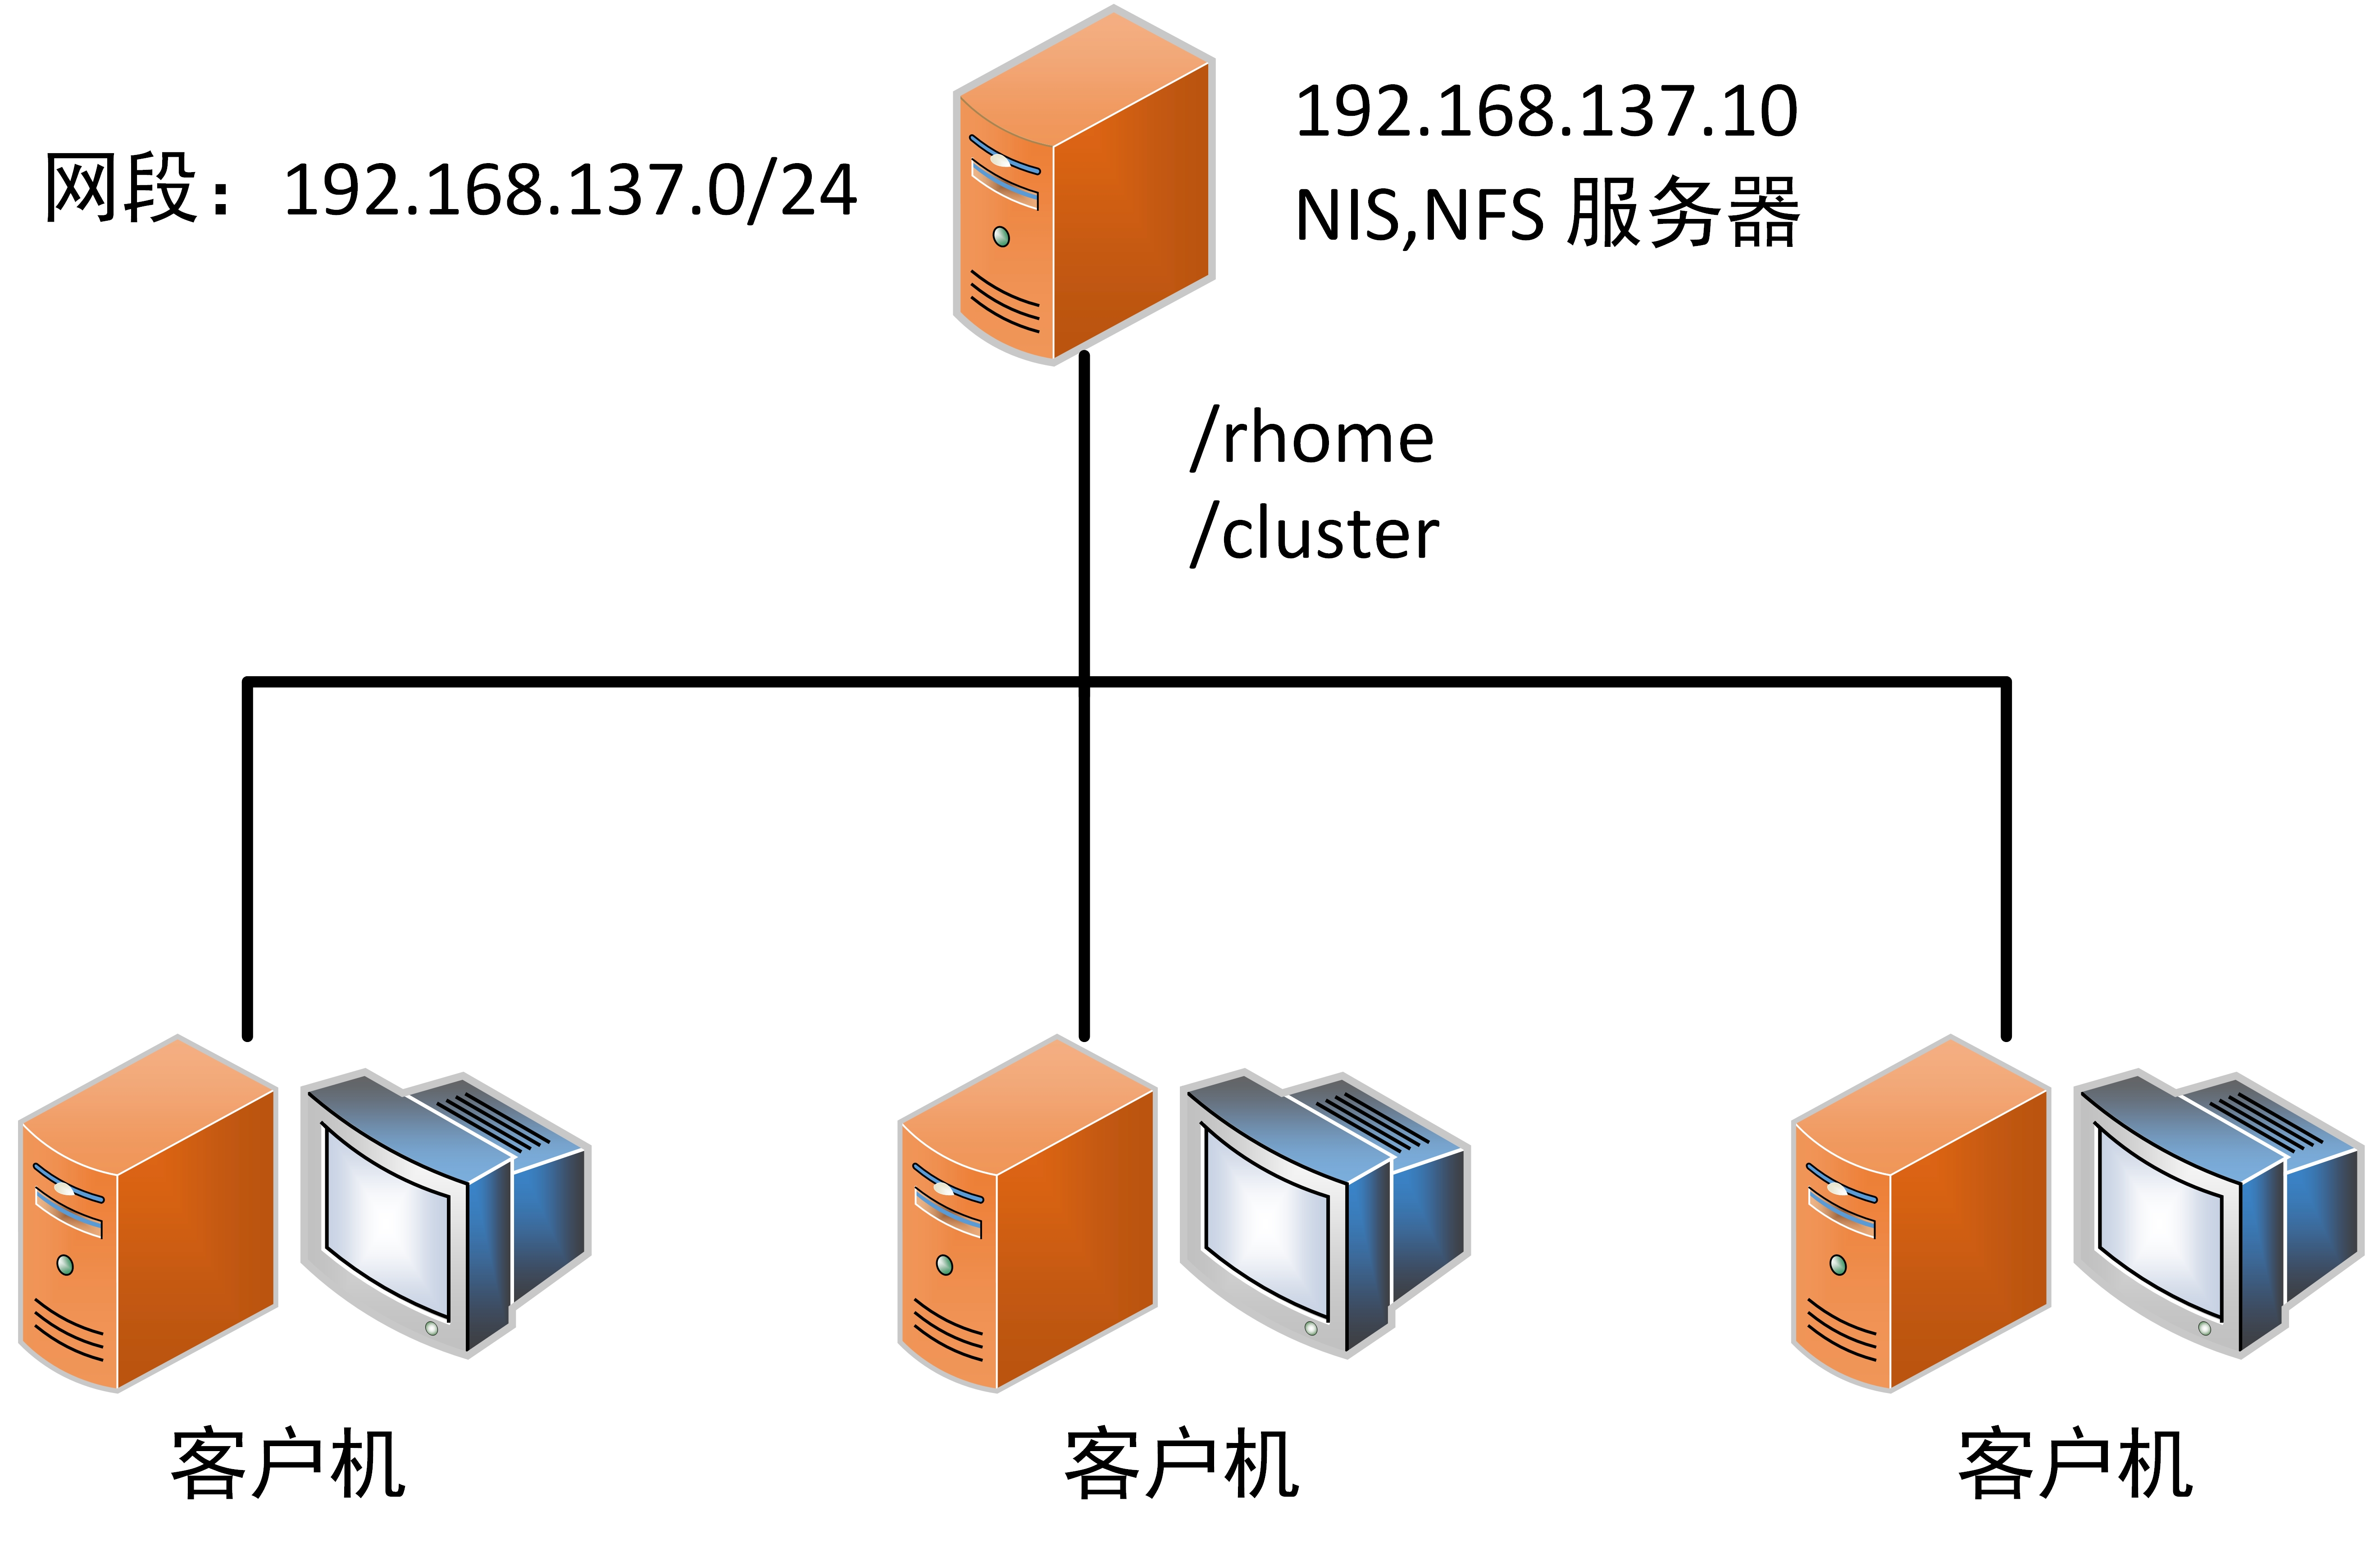
\includegraphics[width=\textwidth]{pic/NIS&NFS.jpg}
\caption{NIS,NFS集群系统}
\end{figure}
建立UID大于2000的账号,账号名为cluser1,cluser2,cluser3, 主目录在/rhome下,新建组clusergroup,将新建的用户加入该组,该组共享文件夹为/cluster. \textbf{目标}:该组人员在任何一台客户机上都能进行自己的工作.

\subsection{配置}
\subsubsection{服务器}
安装: 
\\
\shell{sudo apt-get install nfs-kernel-server nfs-common rpcbind nis -y}
\par
\textbf{1. NIS}
\par
\shell{sudo vim /etc/hosts.deny}
\\\indent 
增加一行:``\texttt{portmap: ALL}".
\par
\shell{sudo vim /etc/hosts.allow}
\\\indent 
增加一行:``\texttt{portmap: 192.168.137.}".
\par
查看本机的主机名并添加到hosts中.
\\
\shell{hostname}\\\indent
或
\\
\shell{cat /etc/hostname}
\par
\shell{sudo vim /etc/hosts}
\\\indent 
增加一行:``\texttt{192.168.137.10   主机名}".
\par
\shell{sudo service rpcbind restart}
\par
\shell{sudo vim /etc/default/nis}
\\\indent 
修改两处:``\texttt{NISSERVER=master}"和``\texttt{NISCLIENT=false}".
\par
\shell{sudo vim /etc/yp.conf}
\\\indent 
添加服务器信息:``\texttt{domain domainName server 主机名}".
\par
domainName就是安装nis时输入的信息,可以直接在 /etc/defaultdomain 中修改,或者运行以下命令修改:
\\
\shell{sudo dpkg-reconfigure nis}
\par
\shell{sudo vim /etc/ypserv.securenets}
\\\indent 
添加客户端所在网段:``\texttt{255.255.255.0   192.168.137.0}".
\par
\shell{sudo vim /var/yp/Makefile}
\\\indent 
修改一行,添加斜体字段:``\texttt{ALL = passwd \textit{shadow} group ...}".
\par
\shell{sudo service ypserv start}
\par
\shell{sudo /usr/lib/yp/ypinit -m}
\par
\shell{sudo service ypserv restart}

\par
\textbf{2. NFS}
\par
\shell{sudo vim /etc/idmapd.conf}
\\\indent 
修改一行:``\texttt{Domain = domainName}".
\par
\shell{sudo vim /etc/default/nfs-common}
\\\indent 
修改一行:``\texttt{NEED\_IDMAPD = YES}".
\par
\shell{sudo service nfs-kernel-server restart}
\par
\shell{sudo service rpcbind restart}

\subsubsection{客户端}
安装:
\\
\shell{sudo apt-get install nfs-common rpcbind nis -y}
\par
\textbf{1. NIS}
\par
\shell{sudo vim /etc/yp.conf}
\par
加入一行:``\texttt{domain domainName server 服务器主机名}".这里的domainName和服务器设置相同.
\par
\shell{sudo vim /etc/nsswitch.conf}
\\\indent
修改几行,添加斜体字段:\\
``\texttt{passwd: compat \textit{nis}}"\\
``\texttt{group: compat \textit{nis}}"\\
``\texttt{shadow: compat \textit{nis}}"\\
``\texttt{hosts: files dns \textit{nis}}"

\par
\textbf{2. NFS}
\par
\shell{sudo vim /etc/hosts.deny}
\\\indent 增加一行:``\texttt{portmap: ALL}".
\par
\shell{sudo vim /etc/hosts.allow}
\\\indent 增加一行:``\texttt{portmap: 192.168.137.10}".
\par
\shell{sudo vim /etc/hosts}
\\\indent 增加一行:``\texttt{192.168.137.10   主机名}".
\par
\shell{sudo vim /etc/idmapd.conf}
\\\indent 修改一行:``\texttt{Domain = domainName}".
\par
\shell{sudo service idmapd restart}
\par
\shell{sudo reboot}

\subsection{搭建}
\subsubsection{服务器}
\par
新建用户并指定主文件夹:\\
\shell{sudo mkdir /rhome}\\
\shell{sudo useradd -u 3001 -d /rhome/cluser1 -m cluser1}\\
\shell{sudo useradd -u 3002 -d /rhome/cluser2 -m cluser2}\\
\shell{sudo useradd -u 3003 -d /rhome/cluser3 -m cluser3}
\par
添加到同一个组:\\
\shell{sudo groupadd clusergroup}\\
\shell{sudo usermod -a -G clusergroup cluser1}\\
\shell{sudo usermod -a -G clusergroup cluser2}\\
\shell{sudo usermod -a -G clusergroup cluser3}
\par
设置该组的公共文件夹,这里要注意的是设置SGID权限:\\
\shell{sudo mkdir /cluster}\\
\shell{sudo chgrp clusergroup /cluster}\\
\shell{sudo chmod 2770 /cluster}
\par
为新建的用户设置密码,并重建YP数据库:\\
\shell{sudo make -C /var/yp}
\par
通过NFS共享到客户端:\\
\shell{sudo vim /etc/exports}
\par
添加两行:\\
``\texttt{/rhome 192.168.137.0/24(rw,no\_root\_squash)}"\\
``\texttt{/cluster 192.168.137.0/24(rw,no\_root\_squash)}"
\par
重启NFS或者重新挂载exports:
\\
\shell{sudo vim exportfs -arv}
\par
验证是否挂载:
\\
\shell{showmount -e localhost}

\subsubsection{客户端}
\par
查看NFS服务器共享情况:
\\
\shell{sudo showmount -e 192.168.137.10}
\par
设置开机挂载:\\
\shell{sudo mkdir /rhome /cluster}\\
\shell{sudo vim /etc/fstab}
\\
\indent 添加两行:\\
``\texttt{192.168.137.10:/rhome /rhome nfs defaults 0 0}"\\
``\texttt{192.168.137.10:/cluster /cluster nfs defaults 0 0}"
\par
\shell{sudo reboot}
\par
接下来,可在客户机上用cluser1等登陆.



\end{document}
